%!TEX program = xelatex
\documentclass[dvipsnames, svgnames,a4paper,11pt]{article}
% ----------------------------------------------------
%   中山大学物理与天文学院本科实验报告模板
%   作者:Huanyu Shi,2019级
%   知乎:https://www.zhihu.com/people/za-ran-zhu-fu-liu-xing
%   Github:https://github.com/huanyushi/SYSU-SPA-Labreport-Template
%   Last update : 2023.4.10
% ----------------------------------------------------

% ----------------------------------------------------- 
%	加边框的命令
%	参考:https://tex.stackexchange.com/questions/531559/how-to-add-the-page-border-for-first-two-pages-in-latex
\usepackage{tikz}
\usetikzlibrary{calc}
\usepackage{eso-pic}
\AddToShipoutPictureBG{%
\begin{tikzpicture}[overlay,remember picture]
\draw[line width=0.6pt] % 边框粗细
    ($ (current page.north west) + (0.6cm,-0.6cm) $)
    rectangle
    ($ (current page.south east) + (-0.6cm,0.6cm) $); % 边框位置
\end{tikzpicture}}


\usepackage{xcolor}
\definecolor{c1}{HTML}{2752C9} % 目录颜色
\definecolor{c2}{RGB}{190,20,83} % 引用颜色

\usepackage{ctex}
\usepackage[top=28mm,bottom=28mm,left=15mm,right=15mm]{geometry}
\usepackage{hyperref} 
\hypersetup{
	colorlinks,
	linktoc = section, % 超链接位置,选项有section, page, all
	linkcolor = c1, % linkcolor 目录颜色
	citecolor = c1  % citecolor 引用颜色
}
\usepackage{amsmath,enumerate,multirow,float}
\usepackage{tabularx}
\usepackage{tabu}
\usepackage{subfig}
\usepackage{fancyhdr}
\usepackage{graphicx}
\usepackage{wrapfig}  
\usepackage{physics}
\usepackage{appendix}
\usepackage{amsfonts}

%
\usepackage{tcolorbox}
\tcbuselibrary{skins,breakable}
\newtcolorbox{tbox}[2][]{
    colframe=black!70!,
    breakable,
    enhanced,
	boxrule =0.5pt,
    title = {#2},
    fonttitle = \large\kaishu\bfseries,
	drop fuzzy shadow,
    #1
}
\newtcolorbox[auto counter,number within=section]{question}[1][]{
  top=2pt,bottom=2pt,arc=1mm,
  boxrule=0.5pt,
%   frame hidden,
  breakable,
  enhanced, %跨页后不会显示下边框
  coltitle=c1!80!gray,
  colframe=c1,
  colback=c1!3!white,
  drop fuzzy shadow,
  title={思考题~\thetcbcounter:\quad},
  fonttitle=\bfseries,
  attach title to upper,
  #1
}

% ---------------------------------------------------------------------
%	利用cleveref改变引用格式,\cref是引用命令
\usepackage{cleveref}
\crefformat{figure}{#2{\textcolor{c2}{图 #1}}#3} % 图片的引用格式
\crefformat{equation}{#2{(\textcolor{c2}{#1})}#3} % 公式的引用格式
\crefformat{table}{#2{\textcolor{c2}{表 #1}}#3} % 表格的引用格式


% ---------------------------------------------------------------------
%	页眉页脚设置
\fancypagestyle{plain}{\pagestyle{fancy}}
\pagestyle{fancy}
\lhead{\kaishu 中山大学物理与天文学院近代物理实验\uppercase\expandafter{\romannumeral1}} % 左边页眉,学院 + 课程
\rhead{\kaishu D4-1 \quad 电子自旋共振实验} % 右边页眉,实验报告标题
\cfoot{\thepage} % 页脚,中间添加页码


% ---------------------------------------------------------------------
%	对目录、章节标题的设置
\renewcommand{\contentsname}{\centerline{\huge 目录}}
\usepackage{titlesec}
\usepackage{titletoc}
% \titleformat{章节}[形状]{格式}{标题序号}{序号与标题间距}{标题前命令}[标题后命令]
\titleformat{\section}{\centering\LARGE\songti}{}{1em}{}

% ---------------------------------------------------------------------
%   listing代码环境设置
\usepackage{listings}
\lstloadlanguages{python}
\lstdefinestyle{pythonstyle}{
backgroundcolor=\color{gray!5},
language=python,
frameround=tftt,
frame=shadowbox, 
keepspaces=true,
breaklines,
columns=spaceflexible,                   
basicstyle=\ttfamily\small, % 基本文本设置,字体为teletype,大小为scriptsize
keywordstyle=[1]\color{c1}\bfseries, 
keywordstyle=[2]\color{Red!70!black},   
stringstyle=\color{Purple},       
showstringspaces=false,
commentstyle=\ttfamily\scriptsize\color{green!40!black},%注释文本设置,字体为sf,大小为smaller
tabsize=2,
morekeywords={as},
morekeywords=[2]{np, plt, sp},
numbers=left, % 代码行数
numberstyle=\it\tiny\color{gray}, % 代码行数的数字字体设置
stepnumber=1,
rulesepcolor=\color{gray!30!white}
}




% ---------------------------------------------------------------------
%	其他设置
\def\degree{${}^{\circ}$} % 角度
\graphicspath{{./images/}} % 插入图片的相对路径
\allowdisplaybreaks[4]  %允许公式跨页 % 导入模板的相关设置
\usepackage{lipsum}
\usepackage{enumitem}
\usepackage{tabularray}  %绘制表格时可以更加方便添加框线
\usepackage{longtable}
\setlist[enumerate]{label=\textup{(\arabic*)}}



%---------------------------------------------------------------------
%	正文
%---------------------------------------------------------------------

\begin{document}


\begin{table}
	\renewcommand\arraystretch{1.7}
	\begin{tabularx}{\textwidth}{
		|X|X|X|X
		|X|X|X|X|}
	\hline
	\multicolumn{2}{|c|}{预习报告}&\multicolumn{2}{|c|}{实验记录}&\multicolumn{2}{|c|}{分析讨论}&\multicolumn{2}{|c|}{总成绩}\\
	\hline
	\LARGE25 & & \LARGE30 & & \LARGE25 & & \LARGE80 & \\
	\hline
	\end{tabularx}
\end{table}


\begin{table}
	\renewcommand\arraystretch{1.7}
	\begin{tabularx}{\textwidth}{|X|X|X|X|}
	\hline
	专业:& 物理学 &年级:& 2022级\\
	\hline
	姓名:& 戴鹏辉 \& 杨舒云  & 学号: & 2344016 \& 22344020 \\
	\hline
	日期:& 2024/10/30 & 教师签名:& \\
	\hline
	\end{tabularx}
\end{table}

\begin{center}
	\LARGE D4-1 \quad 电子自旋共振实验
\end{center}

\textbf{【实验报告注意事项】}
\begin{enumerate}
	\item 实验报告由三部分组成:
	\begin{enumerate}
		\item 预习报告:(提前一周)认真研读\underline{\textbf{实验讲义}},弄清实验原理;实验所需的仪器设备、用具及其使用(强烈建议到实验室预习),完成课前预习思考题;了解实验需要测量的物理量,并根据要求提前准备实验记录表格(第一循环实验已由教师提供模板,可以打印)。预习成绩低于10分(共20分)者不能做实验。
	    \item 实验记录:认真、客观记录实验条件、实验过程中的现象以及数据。实验记录请用珠笔或者钢笔书写并签名(\textcolor{red}{\textbf{用铅笔记录的被认为无效}})。\textcolor{red}{\textbf{保持原始记录,包括写错删除部分,如因误记需要修改记录,必须按规范修改。}}(不得输入电脑打印,但可扫描手记后打印扫描件);离开前请实验教师检查记录并签名。
	    \item 分析讨论:处理实验原始数据(学习仪器使用类型的实验除外),对数据的可靠性和合理性进行分析;按规范呈现数据和结果(图、表),包括数据、图表按顺序编号及其引用;分析物理现象(含回答实验思考题,写出问题思考过程,必要时按规范引用数据);最后得出结论。
	\end{enumerate}
	\textbf{实验报告就是将预习报告、实验记录、和数据处理与分析合起来,加上本页封面。}
	% \item 每次完成实验后的一周内交\textbf{实验报告}(特殊情况不能超过两周)。
	\item 实验安全注意事项
		\begin{enumerate}[label=\roman*.]
			\item 磁极间隙在仪器出厂前已经调整好,实验时最好不要自行调节,以免偏离共振磁场过大。
			\item 双 T 调配器和短路活塞不宜在螺纹范围之外用力调节,避免出现滑丝。
			\item 保护好高斯计探头,避免弯折和挤压。
			\item 励磁电压要缓慢调节,同时仔细注意波形变化,才能辨认出共振吸收峰。
			\item 样品使用时要轻拿轻放,使用完后记得放回样品盒,避免丢失和损坏。
			\item 实验结束后,励磁电压和扫场电压调节到零,再关闭电源,并将所有仪器恢复原状。
		\end{enumerate}
\end{enumerate}


\clearpage
\tableofcontents
\clearpage

\setcounter{section}{0}
\section{D4-1 \quad 电子自旋共振实验 \quad\heiti 预习报告}
	
\subsection{实验目的}
\begin{enumerate}
	\item 了解和掌握各个微波波导器件的功能和调节方法。
	\item 了解电子自旋共振的基本原理,比较电子自旋共振与核磁共振各自的特点。
	\item 观察在微波段电子自旋共振现象,测量 DPPH 样品自由基中电子的朗德因子。
	\item 理解谐振腔中 $\mathrm{TE}_{10}$ 波形成驻波的情况,调节样品腔长,测量不同的共振点,确定波导波长。
	\item 学会利用 DPPH 样品 EPR 共振吸收信号数据拟合法和谱宽直接估测法,获得样品的横向弛豫时间。
	
\end{enumerate}

\subsection{仪器用具}

% \begin{table}[htbp]
% 	\centering
% 	\renewcommand\arraystretch{1.6}
% 	% \setlength{\tabcolsep}{10mm}
% 	\caption{电子自旋共振实验仪器用具}
% 	\begin{tabular}{p{0.05\textwidth}|p{0.20\textwidth}|p{0.05\textwidth}|p{0.5\textwidth}}
% 		\hline
% 		编号& 仪器用具名称 & 数量 &  主要参数(型号,测量范围,测量精度等) \\
% 		\hline
% 		1	&	控制主机 	& 1 & 	\\

% 		2	&	组合式电磁铁 	& 1 & 	 \\
		
% 		3	&	支撑座 & 1 &	 	\\
		
% 		4	&	微波系统	& 1 &  	\\
		
% 		5	&	DPPH 实验样品	& 1 & 玻璃管装	\\

% 		6	&	高斯计探头	& 1 &   \\

% 		7	&	微波源连接线(高频)	& 1 &  	\\

% 		8	&	磁铁电源连接线	& 1 & 红黑各一根	\\

% 		9	&	Q9 连接线	& 1 &  	\\

% 		10	&	三芯航空连接线	& 1 &  	\\

% 		11	&	主机电源线	& 1 &  	\\

% 		11	&	主机电源线	& 1 &  	\\

% 		11	&	主机电源线	& 1 &  	\\

% 		12	&	 短路活塞	& 1 & 属微波系统 	\\

% 		13	&	直波导样品腔	& 1 & 属微波系统 	\\

% 		14	&	扭波导	& 1 & 属微波系统 	\\

% 		15	&	微波频率计	& 1 & 属微波系统 	\\

% 		16	&	双 T 阻抗匹配器	& 1 & 属微波系统 	\\

% 		17	&	环形器	& 1 & 属微波系统 	\\

% 		18	&	检波器	& 1 & 属微波系统 	\\

% 		19	&	隔离器	& 1 & 属微波系统 	\\

% 		20	&	固体微波源	& 1 & 属微波系统 	\\

% 		\hline
% 	\end{tabular}
% 	\label{tbl:电子自旋共振实验仪器用具}
% \end{table}

\begin{longtable}[htbp]{p{0.05\textwidth}|p{0.20\textwidth}|p{0.05\textwidth}|p{0.5\textwidth}}
	\caption{电子自旋共振实验仪器用具} \label{tbl:电子自旋共振实验仪器用具} \\
	\hline
	编号 & 仪器用具名称 & 数量 & 主要参数(型号,测量范围,测量精度等) \\
	\hline
	\endfirsthead
	
	\hline
	编号 & 仪器用具名称 & 数量 & 主要参数(型号,测量范围,测量精度等) \\
	\hline
	\endhead
	
	\hline
	\multicolumn{4}{r}{续下页} \\
	\hline
	\endfoot
	
	\hline
	\endlastfoot
	
	1 & 控制主机 & 1 &  \\
	2 & 组合式电磁铁 & 1 &  \\
	3 & 支撑座 & 1 &  \\
	4 & 微波系统 & 1 &  \\
	5 & DPPH 实验样品 & 1 & 玻璃管装 \\
	6 & 高斯计探头 & 1 &  \\
	7 & 微波源连接线(高频) & 1 &  \\
	8 & 磁铁电源连接线 & 1 & 红黑各一根 \\
	9 & Q9 连接线 & 1 &  \\
	10 & 三芯航空连接线 & 1 &  \\
	11 & 主机电源线 & 1 &  \\
	12 & 短路活塞 & 1 & 属微波系统 \\
	13 & 直波导样品腔 & 1 & 属微波系统 \\
	14 & 扭波导 & 1 & 属微波系统 \\
	15 & 微波频率计 & 1 & 属微波系统 \\
	16 & 双 T 阻抗匹配器 & 1 & 属微波系统 \\
	17 & 环形器 & 1 & 属微波系统 \\
	18 & 检波器 & 1 & 属微波系统 \\
	19 & 隔离器 & 1 & 属微波系统 \\
	20 & 固体微波源 & 1 & 属微波系统 \\
	
\end{longtable}




\clearpage

\subsection{原理概述}

	% \begin{itemize}
	% 	\item \textbf{实验样品:}

	% 		本实验使用的标准样品是DPPH(二苯基苦酸基联氨),其分子式为 $(C_6H_5)_2N - NC_6H_2(NO_2)_3$,含有一个未配对的自由电子。该自由电子只有自旋角动量,未参与轨道角动量,因此可以通过电子自旋共振(ESR)现象进行观察。DPPH中的自由电子不是完全自由的,其g因子的标准值为2.0036,标准线宽为 $2.7 \times 10^{-4} , \text{T}$

	% 		\begin{figure}[H]
	% 			\centering
	% 			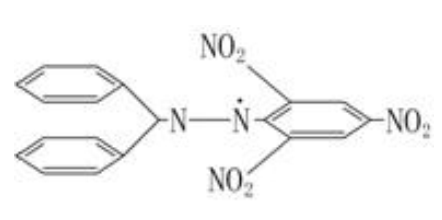
\includegraphics[width=0.4\textwidth]{D4-1-1.png}
	% 			\caption{DPPH 的分子结构式}
	% 			\label{fig:D4-1-1}
	% 		\end{figure}

			

	% 	\item \textbf{电子自旋共振(ESR)与核磁共振(NMR)的比较:}
			
	% 		电子自旋共振(ESR)与核磁共振(NMR)之间的比较主要体现在研究对象、灵敏度和适用范围等方面。ESR 主要关注未偶电子的共振跃迁,而 NMR 则研究磁性核(如质子)的共振跃迁。由于玻尔磁子与核磁子之比,核塞曼能级的裂距较小,使得在相同磁场下,ESR 的频率范围位于微波段。这也导致 ESR 在灵敏度上优于 NMR,能够检测到低至 $10^{-4}$ mol 的样品,尤其适合于半导体中的微量杂质。
		
	% 		在弛豫时间方面,由于电子的磁矩大于核的磁矩,ESR 的顺磁弛豫相互作用较强,导致纵向弛豫时间 $T_1$ 和横向弛豫时间 $T_2$ 较短,从而使谱线通常较宽。虽然 ESR 只能研究与未偶电子相关的局部结构信息,尤其在固体材料的研究中表现突出,但 NMR 在有机化合物分析方面更为优越。值得一提的是,ESR 是唯一直接检测物质中未偶电子的方法,通过吸附、电解、热解等化学反应可以产生顺磁中心,从而实现相关研究。


	% 	\item \textbf{电子自旋共振条件:}
		
	% 		原子中电子的轨道角动量 $P_l$ 和自旋角动量 $P_s$ 会引起相应的轨道磁矩 $\mu_l$ 和自旋磁矩 $\mu_s$,而 $P_l$ 和 $P_s$ 的总角动量 $P_j $ 引起相应的电子总磁矩为 
	% 		\[
	% 			\mu_j = -g \frac{e}{m_e} P_j
	% 		\]
			
	% 		朗德因子 $g$ 由下式计算得到:
	% 		\[
	% 			g = 1 + \frac{J(J + 1) + S(S + 1) - L(L + 1)}{2J(J + 1)}
	% 		\]
	% 		式中 L , S 分别为对原子角动量 J 有贡献的各电子所合成的总轨道角动量和自旋角动量
	% 		量子数。

	% 		通常原子磁矩的单位用波尔磁子 $\mu_B$ 表示,这样原子中的电子的磁矩可以写成
	% 		\[
	% 			\mu_j = -g \frac{\mu_B}{\hbar} P_j = \gamma P_j
	% 		\]

	% 		$\gamma$ 为磁旋比。在外磁场中角动量 $P_j$ 和磁矩 $\mu_j$ 在空间的取向是量子化的。在外磁场方向(Z 轴)的投影为
	% 		\[
	% 			P_z = m \hbar
	% 		\]
	% 		\[
	% 			\mu_z = \gamma m \hbar
	% 		\]

	% 		式中 m 为磁量子数,$m = j, j - 1, ..., - j$ 。当原子磁矩不为零的顺磁物质置于恒定外磁场 $B_0$ 中时,其相互作用能也是不连续的,其相应的能量为
	% 		\[
	% 			E = - \mu_j B_0 = - \gamma m \hbar B_0 = - m g \mu_B B_0
	% 		\]

	% 		不同磁量子数 m 所对应的状态上的电子具有不同的能量。各磁能及是等距分裂的,两相邻磁能级之间的能量差为
	% 		\[
	% 			\Delta E = g \mu_B B_0 = \omega_0 \hbar
	% 		\]
			
	% 		若在垂直于恒定外磁场 $B_0$ 方向上加一交变电磁场,其频率满足 $\omega \hbar = \Delta E $,当 $\omega = \omega_0$ 时,电子在相邻能级间就有跃迁。这种在交变磁场作用下,电子自旋磁矩与外磁场相互作用所产生的能级间的共振吸收(和辐射)现象,称为电子自旋共振(ESR)。

	% 		共振条件可表示为:
	% 		\[
	% 			\omega = g \frac{\mu_B}{\hbar} B_0
	% 		\]

	% 		对于样品 DPPH 来说,朗德因子参考值为 $g = 2.0036$,可得 $f = 2.8043 B_0$,在此 $B_0$ 的单位为高斯,f 的单位为兆赫兹(MHz)。

	% 		% 共振吸收的另一个必要条件是在平衡状态下,低能态 $E_1$ 的粒子数 $N_1$ 比高能态 $E_2$ 的粒子数 $N_2$ 多,这样才能够显示出宏观(总体)共振吸收。

	% 		% 因为热平衡时粒子数分布服从玻尔兹曼分布
	% 		% \[
	% 		% 	\frac{N_1}{N_2} = e^{- \frac{E_2 - E_1}{k T}}
	% 		% \]

	% 		% 因为 $E_2 > E_1$ ,显然有 $N_1 > N_2$ ,即吸收跃迁( $E_1 \rightarrow E_2$ )占优势,然而随着时间推移以及 $E_2 \rightarrow E_1$ 过程的充分进行,势必使 $N_2$ 与 $N_1$ 之差趋于减小,甚至可能反转,于是吸收效应会减少甚至停止,但实际并非如此,因为包含大量原子或离子的顺磁体系中,自旋磁矩之间随时都在相互作用而交换能量,同时自旋磁矩又与周围的其他质点(晶格)相互作用而交换能量,这使处在高能态的电子自旋有机会把它的能量传递出去而回到低能态,这个过程称为弛豫过程,正是弛豫过程的存在,才能维持着连续不断的磁共振吸收效应。



	% 		共振吸收的另一个必要条件是在平衡状态下,低能态 $E_1$ 的粒子数 $N_1$必须大于高能态 $E_2$ 的粒子数 $N_2$。根据玻尔兹曼分布,在热平衡时,粒子数分布遵循关系
	% 		\[
	% 			\frac{N_1}{N_2} = e^{- \frac{E_2 - E_1}{k T}}
	% 		\]
			
	% 		因此当 $E_2 > E_1$ 时,必然有 $N_1 > N_2$ 。这表明吸收跃迁($E_1 \rightarrow E_2$ )占优势。然而,随着时间推移,高能态到低能态的跃迁也会进行,导致 $N_2$ 与 $N_1$的差值减小,甚至可能反转。尽管如此,在包含大量原子或离子的顺磁体系中,自旋磁矩之间会相互作用并交换能量,同时也与周围的晶格相互作用。这种能量传递使得高能态的电子自旋能够将能量释放回到低能态,从而维持连续的磁共振吸收效应。因此,弛豫过程的存在是保证共振吸收持续进行的重要因素。

	% 		弛豫过程所需的时间称为弛豫时间 T,可证明
	% 		\[
	% 			T = \frac{1}{2 T_1} + \frac{1}{T_2}
	% 		\]

	% 		$T_1$ 称为“自旋-晶格弛豫时间”,也称为“纵向弛豫时间”,$T_2$ 称为“自旋-自旋弛豫时间”,也称为“横向弛豫时间”。





	% 	\item \textbf{谱线宽度:}
		
	% 		ESR 谱线具有一定的宽度,用频宽 $\delta \nu $ 表示,与能量差 $\Delta E$ 相关,公式为 $\delta \nu = \frac{\Delta E}{h}$ 。根据测不准原理,能级寿命 $\tau$ 与能量的不确定量 $\delta E$ 存在关系 $\tau \delta E \sim h $,因此 $\tau \delta \nu \sim 1$,这表明粒子在高能级的寿命缩短会导致谱线加宽。
		
	% 		谱线宽度的主要原因是自旋-晶格相互作用和自旋-自旋相互作用,其中对于大多数自由基,自旋-自旋相互作用起主导作用。这种相互作用涉及未偶电子与相邻原子核自旋之间的相互作用,以及两个分子间未偶电子的相互作用。因此,谱线宽度反映了粒子间相互作用的信息,成为电子自旋共振谱的重要参数。
		
	% 		通过移相器信号作为示波器扫描信号,可以测定吸收峰的半高宽 $\Delta B$(谱线宽度)。若谱线呈洛伦兹型,可以用公式 $\Delta B = \frac{2 \gamma }{T}$ 计算,其中 $\gamma$ 为旋磁比,进而求得共振样品的横向弛豫时间 $T_2$。

		

	% 	\item \textbf{微波基础知识与微波套件:}
		
	% 		\begin{enumerate}
	% 			\item \textbf{微波及其传输}
	% 			\begin{enumerate}
	% 				\item 由于微波的波长短,频率高,它已经成为一种电磁辐射,所以传输微波就不能用一般的金属导线。
	% 				\item 常用的微波传输器件有同轴线、波导管、带状线和微带线等,引导电磁波传播的空心金属管称为波导管。
	% 				\item 常见的波导管有矩形波导管和圆柱形波导管两种。
	% 				\item 在波导中只能存在下列两种电磁波:
	% 				\begin{itemize}
	% 					\item TE 波,即横电波,它的电场只有横向分量而磁场有纵向分量;
	% 					\item TM 波,即横磁波,它的磁场只有横向分量而电场存在纵横分量。
	% 				\end{itemize}
	% 				\item TE10 波是矩形波导中最简单和最常使用的一种波型,也称为主波型。
	% 				\item 沿 z 方向传播的 TE10 波的各分量为:
	% 				\begin{align}
	% 					E_y &= E_0 \sin\left(\frac{\pi x}{a}\right) e^{i(\omega t - \beta z)} \\
	% 					H_x &= \frac{E_0}{\omega \mu} \sin\left(\frac{\pi x}{a}\right) e^{i(\omega t - \beta z)} \\
	% 					H_z &= \frac{E_0}{\omega \mu} \cos\left(\frac{\pi x}{a}\right) e^{i(\omega t - \beta z)}
	% 				\end{align}
	% 				\item 其中 $\beta = \frac{2\pi}{\lambda_g}$ 称为相位常数,$\lambda_g$ 称为波导波长,$\lambda_c = 2a$ 为截止波长。
	% 				\item TE10 波的特性包括:
	% 				\begin{itemize}
	% 					\item 只有波长 $\lambda < \lambda_c$ 的电磁波才能在波导管中传播;
	% 					\item 电场矢量垂直于波导宽壁,沿 $x$ 方向两边为 0,中间最强,沿 $y$ 方向是均匀的。
	% 				\end{itemize}
	% 			\end{enumerate}
			
	% 			\item \textbf{微波器件}
	% 			\begin{enumerate}
	% 				\item \textbf{固态微波信号源}
	% 				\begin{itemize}
	% 					\item 常用的微波振荡器有反射式速调管振荡器和耿式二极管振荡器。
	% 					\item 耿式二极管的核心是基于 n 型砷化镓的导带双谷结构。
	% 				\end{itemize}
					
	% 				\item \textbf{隔离器}
	% 				\begin{itemize}
	% 					\item 隔离器是一种不可逆的衰减器,正方向衰减量小,反方向衰减量大。
	% 					\item 可避免因负载变化使微波源的频率及输出功率发生变化。
	% 				\end{itemize}
			
	% 				\item \textbf{环行器}
	% 				\begin{itemize}
	% 					\item 三端口环行器用于定向传输电磁波。
	% 					\item 内装有圆柱形铁氧体柱,并施加恒磁场以产生场移效应。
	% 				\end{itemize}
			
	% 				\item \textbf{晶体检波器}
	% 				\begin{itemize}
	% 					\item 使用半导体点接触二极管检波微波信号。
	% 				\end{itemize}
			
	% 				\item \textbf{双 T 调配器}
	% 				\begin{itemize}
	% 					\item 用于使微波部件调成匹配,避免反射。
	% 					\item 具有宽频带和驻波匹配范围的优点。
	% 				\end{itemize}
			
	% 				\item \textbf{频率计}
	% 				\begin{itemize}
	% 					\item 吸收式谐振频率计用于测量微波频率。
	% 				\end{itemize}
			
	% 				\item \textbf{扭波导}
	% 				\begin{itemize}
	% 					\item 用于改变电磁波的偏振方向以便于机械安装。
	% 				\end{itemize}
			
	% 				\item \textbf{矩形谐振腔}
	% 				\begin{itemize}
	% 					\item 由一段矩形波导和封闭金属片组成,形成反射式谐振腔。
	% 				\end{itemize}
			
	% 				\item \textbf{短路活塞}
	% 				\begin{itemize}
	% 					\item 接在传输系统终端的单臂微波元件,用于形成驻波状态。
	% 				\end{itemize}
	% 			\end{enumerate}
	% 		\end{enumerate}









	% \end{itemize}
	\begin{enumerate}
		\item DPPH
		
		结构式如\cref{fig:dpph}所示。它的第 2个 N 原子少了一个共价键,有一个未偶电子,或者说一个未配对的“自由电子”,是一个稳定的有机自由基。对于这种自由电子,它只有自旋角动量而没有轨道角动量。或者说它的轨道角动量完全猝灭了。所以在实验中能够容易地观察到 ESR 现象。
		
		\begin{figure}[h!]
			\centering
			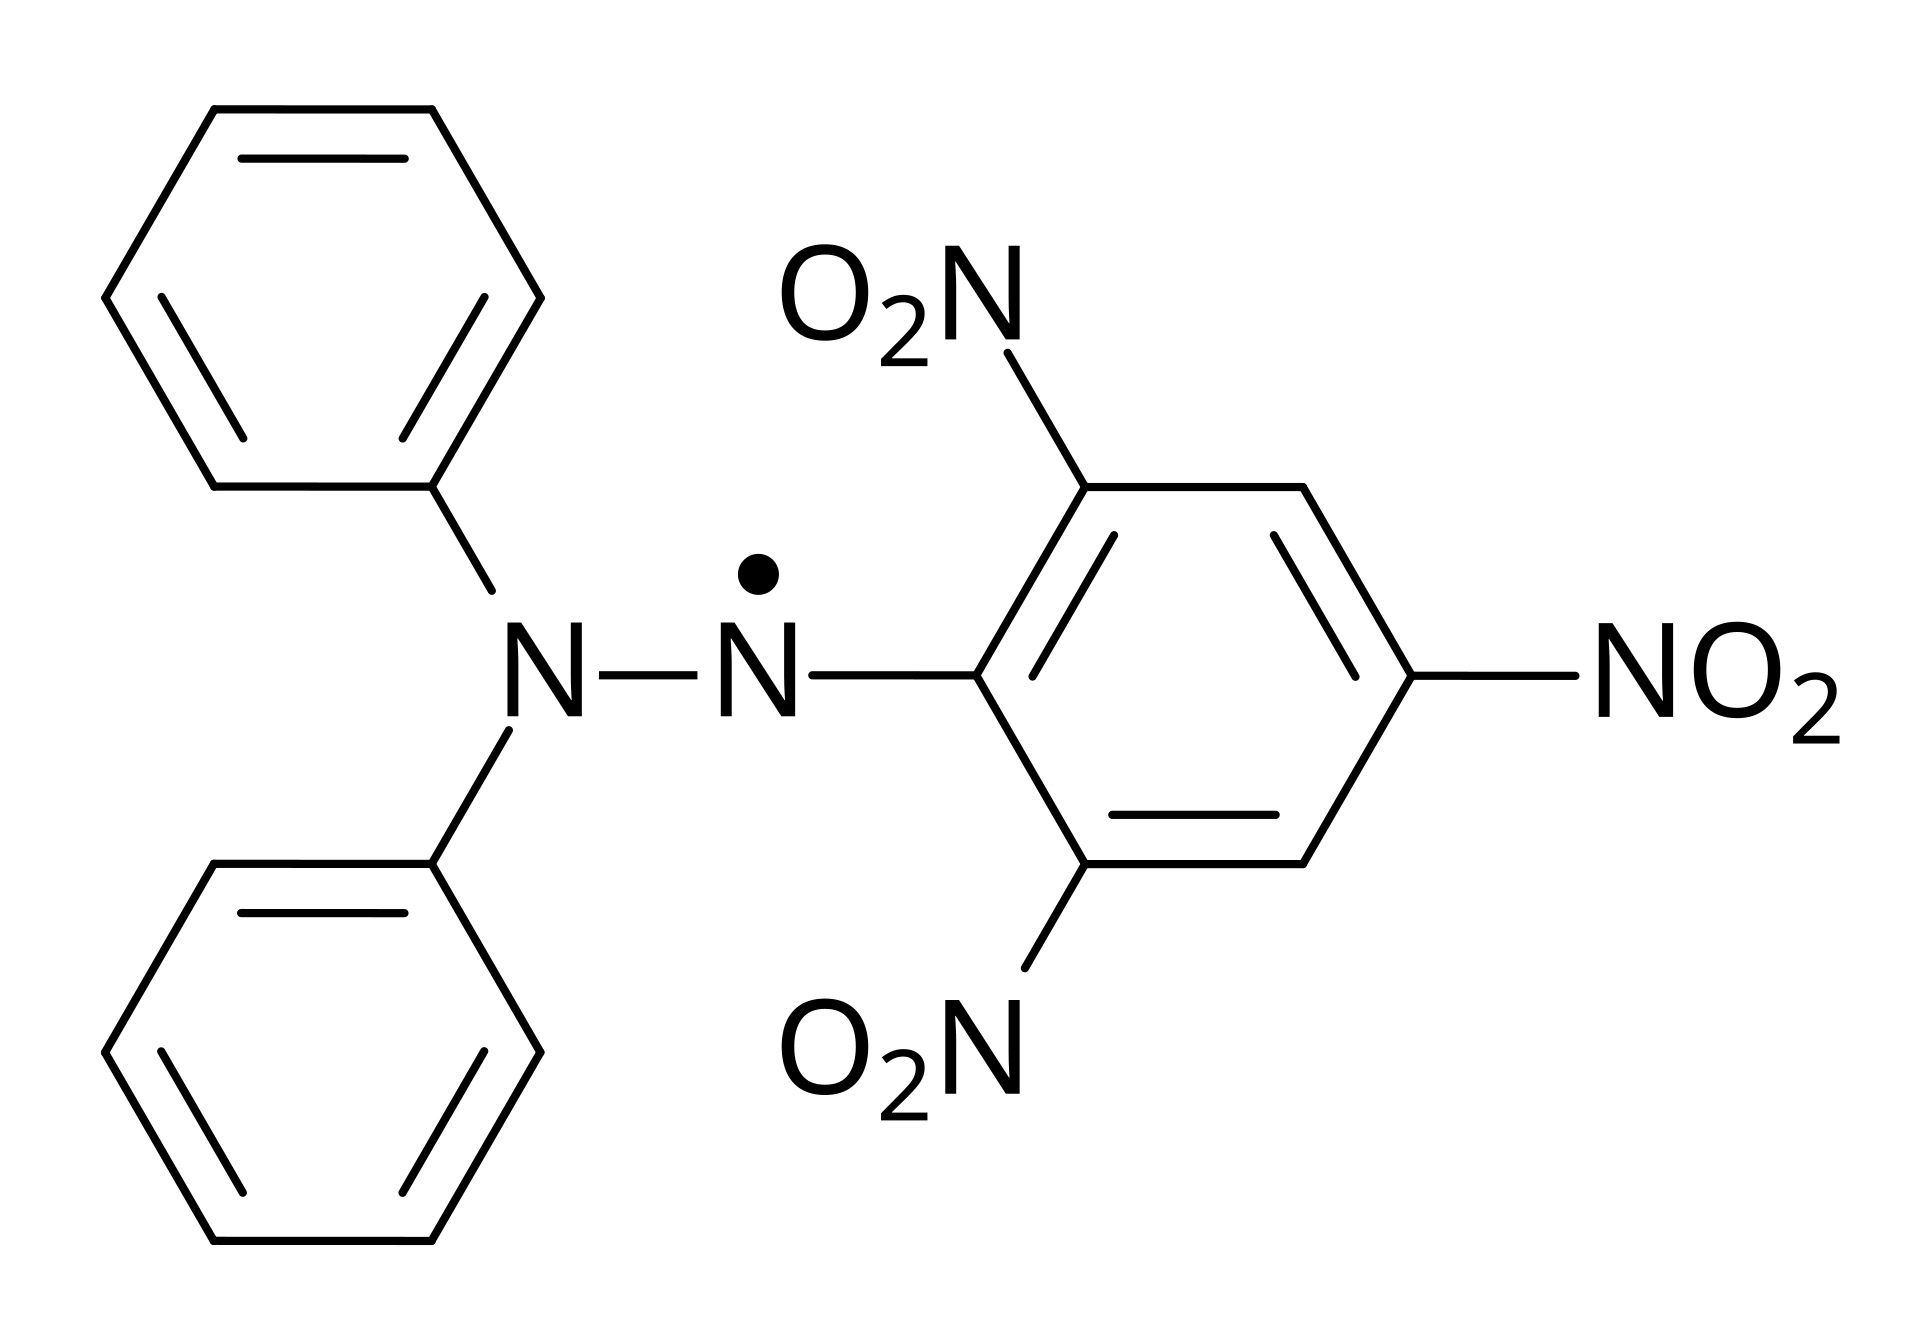
\includegraphics[width=0.4\linewidth]{images/DPPH}
			\caption{2,2-二苯基-1-苦基肼自由基的结构式}
			\label{fig:dpph}
		\end{figure}
		
		由于 DPPH 分子中的“自由电子”并不是完全自由的,其郎德 g 因子标准值为 2.0036,标准线宽为 $2.7\times10^{-4}$T。
		
		\item 电子顺磁共振(EPR)简介
		
		电子顺磁共振(Electron Paramagnetic Resonance, EPR)是一种用于研究具有未成对电子的分子、离子和固体的电子自旋态的方法。这些未成对电子的自旋与外加磁场相互作用,会产生特定的能级分裂,通过吸收或发射微波,可以检测到电子自旋翻转的共振现象。EPR是研究自由基、过渡金属离子以及缺陷中心等系统的强有力工具。
		
		在EPR中,未成对电子的自旋(用自旋角动量算符 \( \mathbf{S} \) 表示)在外加磁场 \( \mathbf{B} \) 下会与磁场发生相互作用。其哈密顿量 \( H \) 可以表示为:\[ H = g \mu_B \mathbf{B} \cdot \mathbf{S} \]其中,\( g \) 是电子自旋的 \( g \) 因子(通常约为2.0023,对于自由电子),\( \mu_B \) 是玻尔磁子,定义为 \( \mu_B = \frac{e \hbar}{2m_e} \),\( \mathbf{B} \) 是外加磁场的矢量,而 \( \mathbf{S} \) 是电子自旋角动量算符。当外加磁场沿 \( z \) 轴施加时,哈密顿量可以简化为:\[ H = g \mu_B B_z S_z \]其中 \( B_z \) 是磁场在 \( z \) 方向的分量,\( S_z \) 是自旋在 \( z \) 方向的分量。该哈密顿量表明,电子的能量将因磁场的存在而发生劈裂,产生两个能级。
		
		在磁场 \( B \) 下,电子的两个自旋态 \( m_s = +\frac{1}{2} \) 和 \( m_s = -\frac{1}{2} \) 对应的能量分别为:\[ E_{\pm} = \pm \frac{1}{2} g \mu_B B \]能量差 \( \Delta E \) 为:\[ \Delta E = g \mu_B B \]这个能量差正是我们在EPR中探测到的共振频率。为了使电子发生自旋跃迁,需要满足电子的能量差与微波辐射的频率相匹配的条件,即共振条件。共振频率 \( \nu \) 满足:\[ h \nu = \Delta E = g \mu_B B \]即\[ \nu = \frac{g \mu_B B}{h} \]其中 \( h \) 为普朗克常数。通过调节外加磁场 \( B \) 或微波频率 \( \nu \),可以找到满足该条件的共振点,从而检测到EPR信号。
		
		% 对于带有核自旋的系统,电子自旋与核自旋之间的相互作用称为超精细相互作用。这种相互作用会导致EPR谱线的进一步分裂,称为超精细分裂。超精细相互作用哈密顿量可以写为:\[ H_{\text{hf}} = \mathbf{I} \cdot \mathbf{A} \cdot \mathbf{S} \]其中 \( \mathbf{I} \) 是核自旋角动量算符,\( \mathbf{A} \) 是超精细张量。这种相互作用会使得每个电子自旋态根据核自旋的取向进一步分裂,从而在EPR谱中产生多个峰。
		
		在实验中,将样品置于磁场和微波场中,逐步调节磁场强度,记录不同磁场下微波吸收的变化。当外加磁场满足共振条件时,样品会吸收特定频率的微波,从而检测到吸收峰。通过分析这些吸收峰的特征,可以获得样品中电子自旋的特性及其与核的相互作用信息。EPR在化学、生物学和物理学中有广泛应用,如探测自由基的结构与反应活性、研究金属离子配合物的电子结构、研究固体材料中的晶格缺陷以及生物大分子中金属离子活性位点的研究。EPR提供的电子和核相互作用信息可以揭示样品的微观结构和局部环境。
		
		\item EPR信号的起源与共振条件
		
		每个电子都有一个\textbf{磁矩}和\textbf{自旋量子数}$s = \tfrac{1}{2}$,其磁性分量为$m_\mathrm{s} = + \tfrac{1}{2}$或$m_\mathrm{s} = - \tfrac{1}{2}$。在外部磁场$B_0$的作用下,电子的磁矩会与磁场平行($m_\mathrm{s} = + \tfrac{1}{2}$)或反平行($m_\mathrm{s} = - \tfrac{1}{2}$)排列,每种排列因\textbf{塞曼效应}具有特定的能量:
		\begin{equation*}
			E = m_s g_e \mu_\text{B} B_0,
		\end{equation*}
		其中:
		\begin{itemize}
			\item $g_e$是电子的\textbf{g因子}(也称\textbf{朗德g因子}),对于自由电子,$g_\mathrm{e} = 2.0023$;
			\item $\mu_\text{B}$是\textbf{玻尔磁子}。
		\end{itemize}
		
		因此,对于未配对的自由电子,高低能态之间的能量差为$\Delta E = g_e \mu_\text{B} B_0$。此方程表明(由于$g_e$和$\mu_\text{B}$是常数),能级的分裂与磁场的强度成正比,如\cref{fig:eprsplitting}所示。
		
		\begin{figure}[h!]
			\centering
			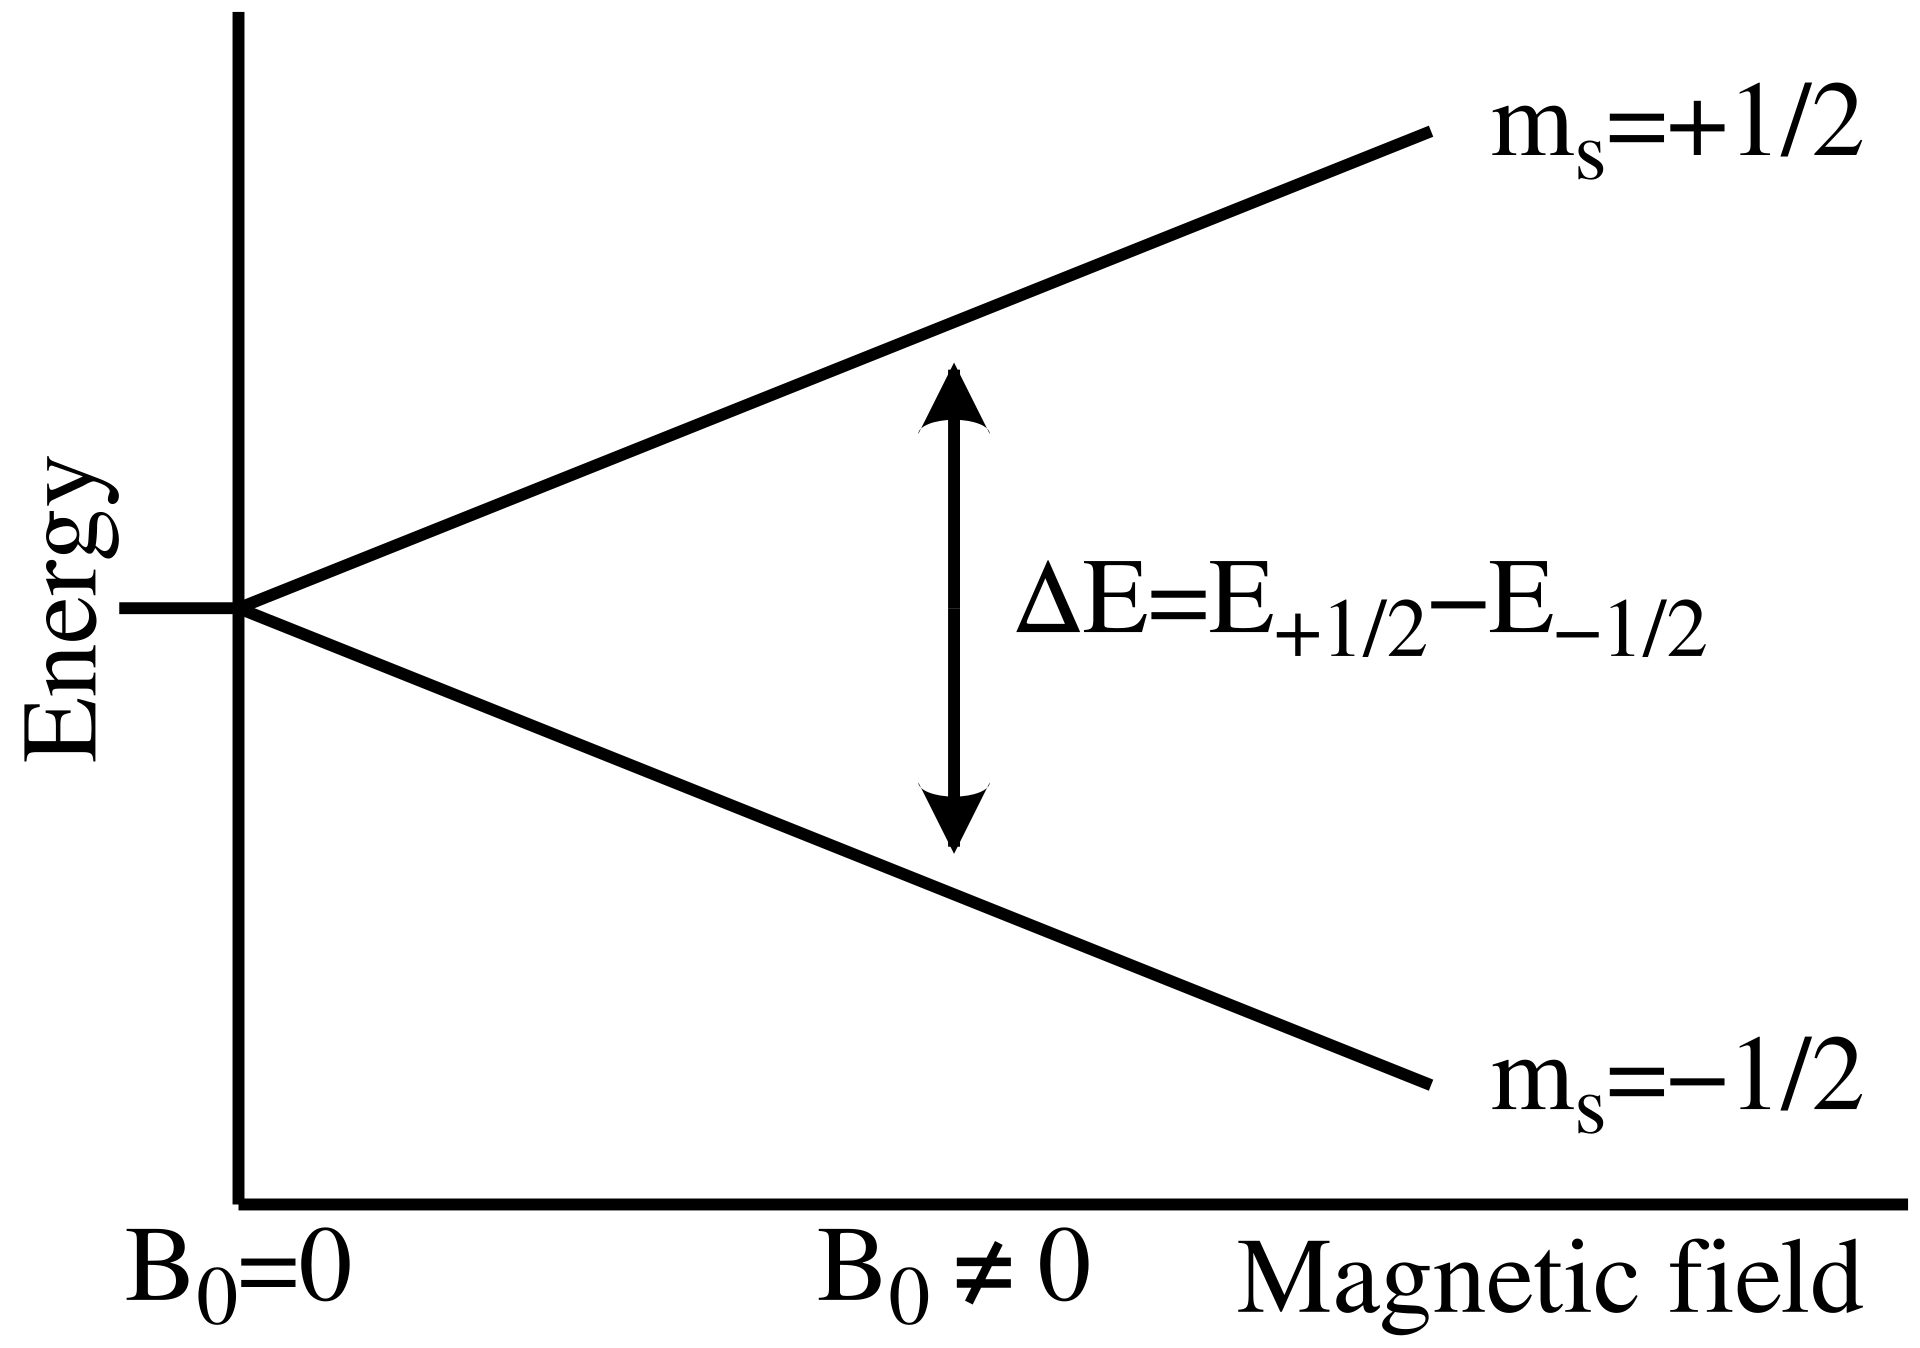
\includegraphics[width=0.5\linewidth]{images/EPR_splitting}
			\caption{电子自旋态的分裂}
			\label{fig:eprsplitting}
		\end{figure}
		
		% \begin{ubox}{}
		% 	未配对的电子可以通过吸收或发射一个能量为$h \nu$的\textbf{光子}来改变其电子自旋,以满足共振条件$h \nu = \Delta E$。这就是EPR光谱学的基本方程:$h \nu = g_e \mu_\text{B} B_0$。
		% \end{ubox}
		未配对的电子可以通过吸收或发射一个能量为$h \nu$的\textbf{光子}来改变其电子自旋,以满足共振条件$h \nu = \Delta E$。这就是EPR光谱学的基本方程:$h \nu = g_e \mu_\text{B} B_0$。
		
		实验上,此方程允许频率和磁场值的多种组合,但大多数EPR测量是在9000-10000 MHz(9-10 GHz)区域的微波下进行,对应的磁场约为3500高斯(0.35 T)。此外,可以通过改变样品上光子的频率并保持磁场恒定,或者反之来生成EPR谱。在实际操作中,通常保持频率恒定。一组\textbf{顺磁}中心(如自由基)暴露在固定频率的微波下。通过增加外部磁场,$m_\mathrm{s} = + \tfrac{1}{2}$和$m_\mathrm{s} = - \tfrac{1}{2}$能态之间的能量差逐渐扩大,直到它匹配微波的能量,如\cref{fig:eprsplitting}中的双箭头所示。此时,未配对电子可以在两个自旋态之间跃迁。由于麦克斯韦-玻尔兹曼分布的关系,通常低能态中的电子数更多,从而产生净能量吸收,监测这种吸收并将其转换为光谱。\cref{fig:eprsignalharmonics}中的上方光谱是一个在变化的磁场下自由电子系统的模拟吸收谱,下方光谱是吸收谱的一阶导数。后一种方式是记录和发布连续波EPR谱的最常用方式。
		
		\begin{figure}[h!]
			\centering
			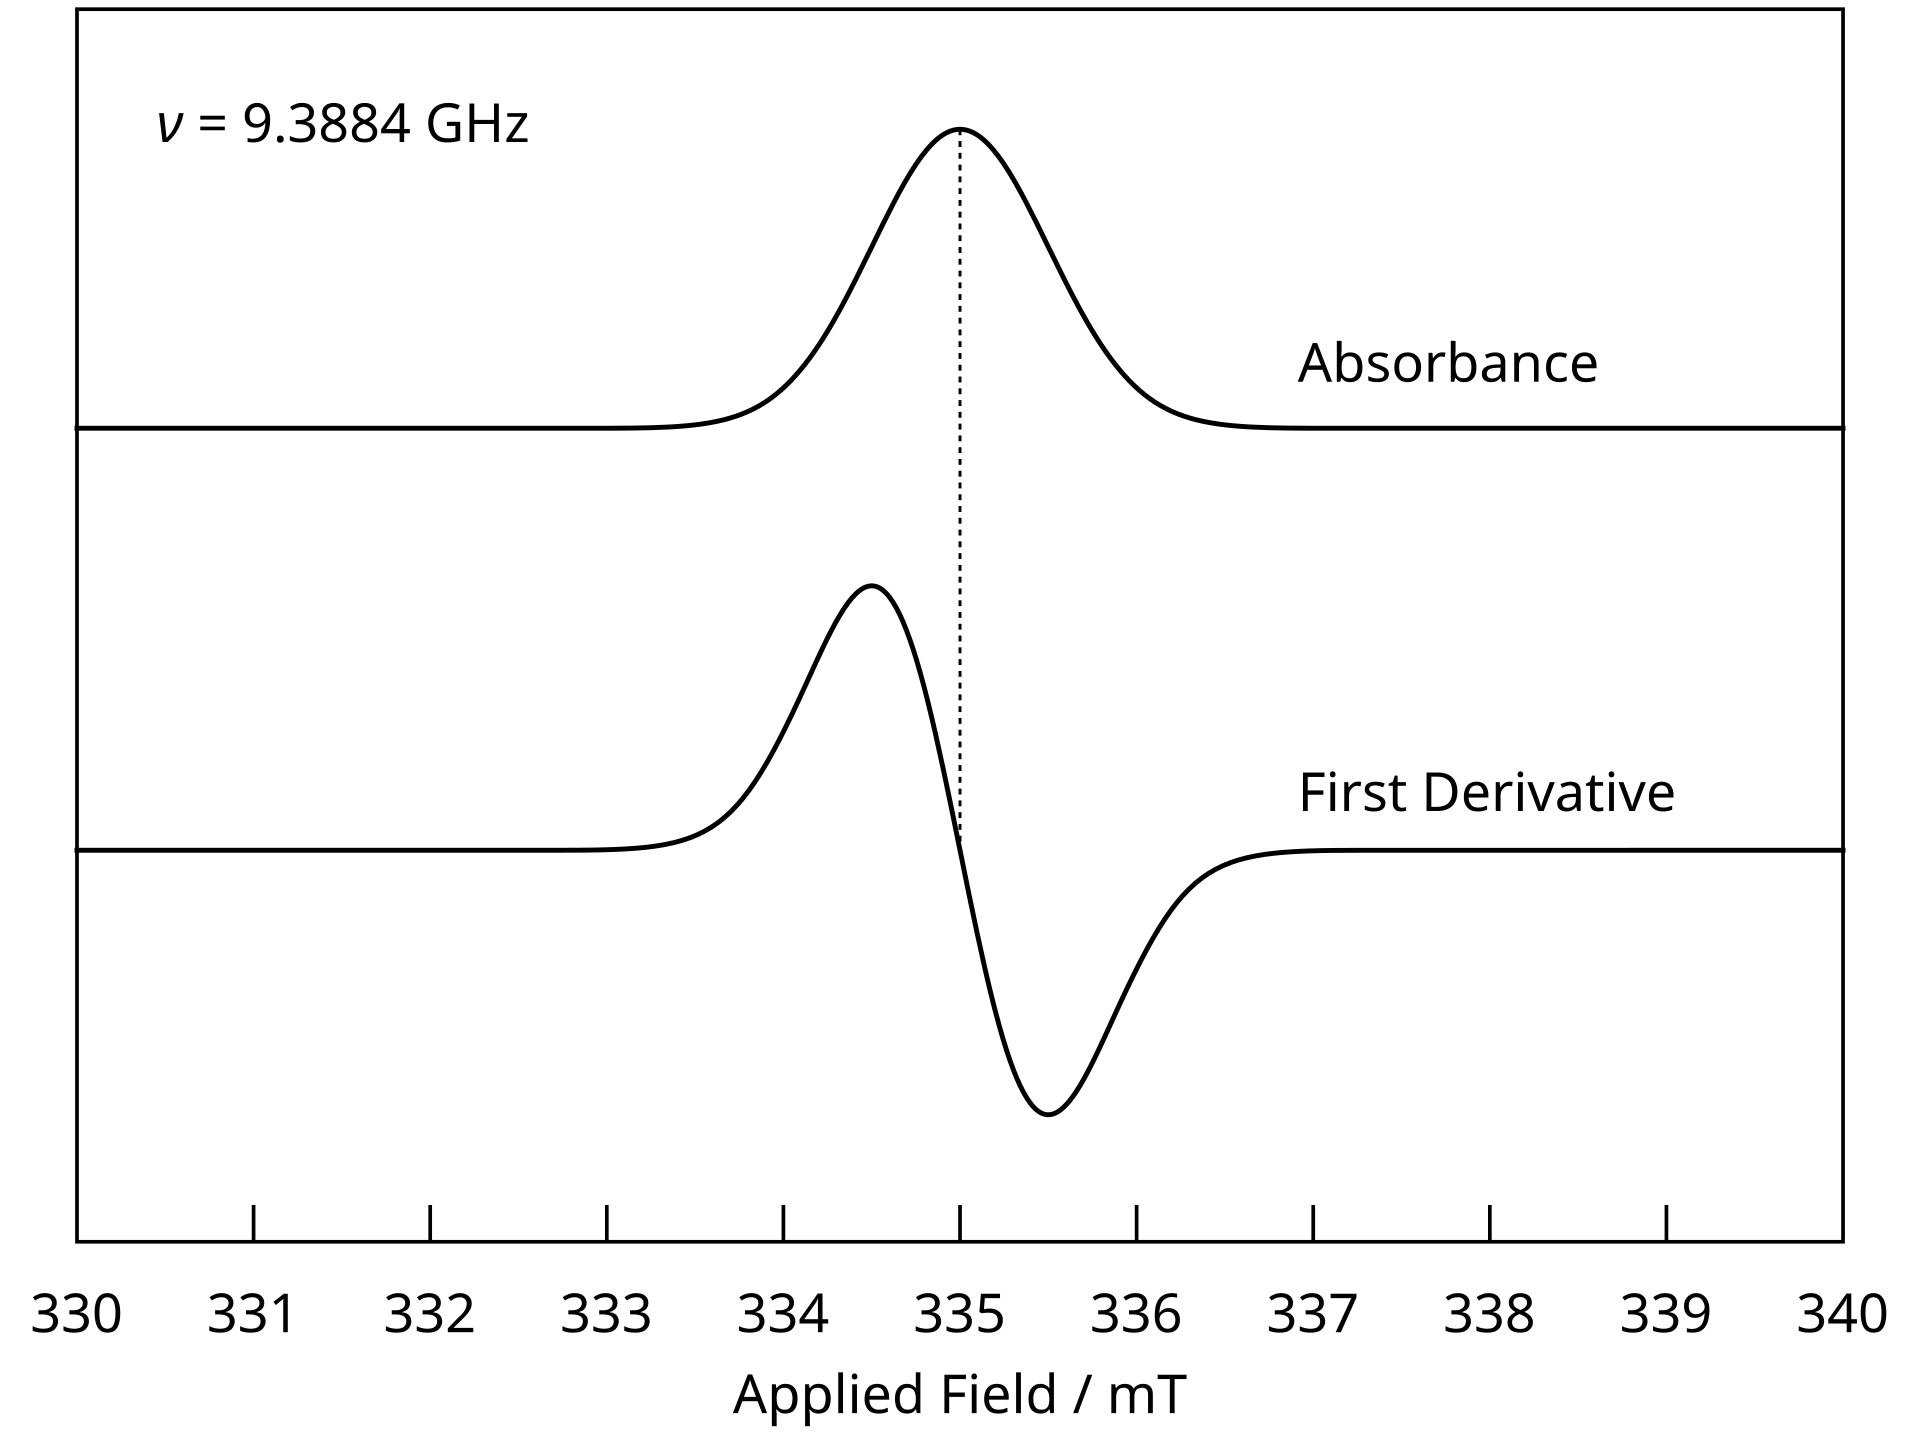
\includegraphics[width=0.5\linewidth]{images/EPR_Signal_Harmonics}
			\caption{在 X 波段频率为 9.3884 GHz 且导数峰峰线宽为 1 mT 时,g = 2.0023 的双峰的吸收和一阶导数 EPR 信号}
			\label{fig:eprsignalharmonics}
		\end{figure}
		
		对于9388.4 MHz的微波频率,预测的共振磁场约为
		\begin{equation*}
			B_0 = \frac{h \nu}{g_e \mu_\text{B}} = 0.3350 \, \text{T} = 3350 \, \text{G} \, .
		\end{equation*}
		
		由于电子与核的质量差异,电子的\textbf{磁矩}远大于任何核的相应值,因此在相同的磁场强度下,需要更高的电磁频率才能引起电子的自旋共振。例如,对于\cref{fig:eprsignalharmonics}中的3350 G磁场,电子的自旋共振发生在约9388.2 MHz,而对于$^1$H核则仅约为14.3 MHz。(对于NMR光谱学,相应的共振方程为$h \nu = g_\mathrm{N} \mu_\mathrm{N} B_0$,其中$g_\mathrm{N}$和$\mu_\mathrm{N}$取决于研究的核种。)
		
		\item 微波及微波器件简介
		
		微波是频率范围在 300 MHz 至 300 GHz 之间的电磁波,其波长范围从1米到1毫米。微波在通讯、雷达、医学、微波加热等领域中有着广泛的应用。在电子顺磁共振(EPR)实验中,微波用于引发电子自旋共振,因为其频率正好能满足未成对电子在外加磁场中自旋跃迁所需的能量差。为实现微波的产生、传输和控制,微波器件发挥了至关重要的作用。
		
		% 微波是一种横波,包含电场和磁场分量。微波在自由空间中传播时,其电磁波方程描述了电场 \( E \) 和磁场 \( H \) 随时间和空间的变化。其基本形式为:\[ \nabla^2 E - \frac{1}{c^2} \frac{\partial^2 E}{\partial t^2} = 0 \]和\[ \nabla^2 H - \frac{1}{c^2} \frac{\partial^2 H}{\partial t^2} = 0 \]其中,\( c \) 是光速。通过这些方程,可以推导出微波在不同介质中的传播特性。微波的频率与电磁波的波长 \( \lambda \) 关系为:\[ \lambda = \frac{c}{f} \]其中 \( f \) 是微波的频率。微波的高频特性使其易于受到物质表面的反射、折射和吸收,因此需要特殊的传输结构和器件来实现有效传输和控制。
		
		微波器件主要包括微波源、波导、滤波器、耦合器、衰减器、放大器和天线等。微波源是用于产生微波信号的器件,常见的微波源包括磁控管、行波管(TWT)和速调管(Klystron)。以磁控管为例,其基本工作原理是通过电场与磁场的作用加速电子产生微波辐射。磁控管的输出频率由其谐振腔结构决定,通常工作在固定频率,广泛应用于微波加热(如微波炉)和雷达中。波导是一种用于传输微波的结构,其作用相当于光纤在光通信中的作用。波导通常是空心的金属管,内部电场和磁场的模式决定了微波在其中的传播模式。波导方程为:\[ \frac{d^2 E_x}{dx^2} + \frac{d^2 E_y}{dy^2} + \left( k^2 - \frac{\omega^2}{c^2} \right) E_z = 0 \]该方程描述了不同模式(如 TE 模式和 TM 模式)下电磁场的分布。波导在低损耗传输微波信号方面具有优势,广泛用于高频应用。
		
		滤波器用于控制特定频段的微波通过,去除不需要的频率分量。常见的微波滤波器包括带通滤波器和带阻滤波器。耦合器则用于实现微波信号的功率分配或合并,其设计基于微波的干涉原理,如分支耦合器、定向耦合器等。衰减器用于减少微波信号的强度,提供精确的信号调节。放大器用于增强微波信号,通常采用行波管放大器(TWT)和半导体放大器。行波管放大器通过电子流与微波信号的相互作用放大信号,而半导体放大器则利用微波频率的电流放大效应。天线用于将微波信号转化为电磁波并发射到空间中。常见的微波天线有抛物面天线、喇叭天线等,天线的辐射效率和方向性决定了其在信号发射与接收中的性能。
		
		% 微波器件通常使用S参数(散射参数)来描述其传输特性。对于一个输入信号 \( a_i \),S参数定义为:\[ S_{ij} = \frac{b_j}{a_i} \]其中 \( b_j \) 为输出信号。S参数可以用于描述信号的反射、透射以及传输损耗等特性。例如,\( S_{11} \) 表示输入端反射,\( S_{21} \) 表示从输入端到输出端的传输特性。
		
		在电子顺磁共振实验中,微波器件如波导、腔体和天线被用来产生并传输微波信号。微波频率在EPR实验中非常关键,因为它需与外加磁场产生的电子能级劈裂频率相匹配,满足共振条件,从而激发电子自旋翻转并产生EPR信号。微波源通过精确的调节和控制,可以产生不同频率的微波,以便与不同的电子能级结构共振,从而揭示样品中电子自旋的微观特性。
	\end{enumerate}



\clearpage
\subsection{实验前思考题}

% 思考题1
\begin{question}
	简述电子自旋共振的基本原理,并与核磁共振作比较。
\end{question}

% \begin{enumerate}
%     \item \textbf{电子自旋共振的基本原理}
%     \begin{enumerate}
%         \item \textbf{自旋与磁矩}:
%         \begin{itemize}
%             \item 电子具有自旋量子数为 \( \frac{1}{2} \),自旋导致电子产生一个磁矩。
%             \item 在外磁场 \( B_0 \) 的作用下,电子的自旋态会分裂为两个能级,能量差与外磁场强度成正比。
%         \end{itemize}

%         \item \textbf{激发与共振}:
%         \begin{itemize}
%             \item 当施加一个与自旋能级差相匹配的电磁辐射(通常在微波范围)时,电子可以从低能态跃迁到高能态,产生共振。
%             \item 共振频率 \( \nu \) 与外磁场强度 \( B_0 \) 之间的关系由朗德公式给出:
%             \[
%             \nu = g \frac{e}{2\pi m_e} B_0
%             \]
%             其中 \( g \) 是朗德因子,\( e \) 是电子电荷,\( m_e \) 是电子质量。
%         \end{itemize}

%         \item \textbf{应用}:
%         \begin{itemize}
%             \item ESR 常用于研究自由基、金属离子及其与环境的相互作用等。
%         \end{itemize}
%     \end{enumerate}

%     \item \textbf{与核磁共振的比较}
%     \begin{enumerate}
%         \item \textbf{探测对象}:
%         \begin{itemize}
%             \item \textbf{ESR}:探测电子的自旋状态,适用于研究具有未成对电子的物质。
%             \item \textbf{NMR}:探测原子核的自旋状态,适用于研究含有核磁性原子(如氢、碳、氮等)的物质。
%         \end{itemize}

%         \item \textbf{频率范围}:
%         \begin{itemize}
%             \item \textbf{ESR}:通常在微波频率范围(几 GHz)。
%             \item \textbf{NMR}:通常在射频频率范围(几十 MHz到几 GHz)。
%         \end{itemize}

%         \item \textbf{外磁场强度}:
%         \begin{itemize}
%             \item \textbf{ESR}:所需的外磁场强度相对较小,一般在几百高斯(0.01 T 左右)。
%             \item \textbf{NMR}:需要较强的外磁场,通常在几特斯拉(T)范围。
%         \end{itemize}

%         \item \textbf{信号强度}:
%         \begin{itemize}
%             \item \textbf{ESR}:由于电子的磁矩大于核的磁矩,因此信号通常较强。
%             \item \textbf{NMR}:信号较弱,通常需要增强技术(如核自旋极化)来提高信号强度。
%         \end{itemize}

%         \item \textbf{应用领域}:
%         \begin{itemize}
%             \item \textbf{ESR}:广泛应用于化学、物理和生物学等领域,特别是自由基和缺陷的研究。
%             \item \textbf{NMR}:广泛应用于化学结构解析、生物分子研究及医学成像(MRI)。
%         \end{itemize}
%     \end{enumerate}
% \end{enumerate}
	
电子自旋共振(Electron Spin Resonance, ESR)或电子顺磁共振(Electron Paramagnetic Resonance, EPR)的基本原理是研究具有未成对电子的原子、离子或分子在外加磁场下的自旋行为。当未成对电子处于磁场中时,其自旋状态会发生能级分裂,称为塞曼分裂,能量差与磁场强度成正比。通过引入与电子能级分裂频率相匹配的微波辐射,可以引发电子自旋的跃迁(即从一个自旋状态翻转至另一个状态)。这种电子自旋翻转会产生微波吸收,从而被检测到作为ESR信号。

与核磁共振(Nuclear Magnetic Resonance, NMR)相比,ESR和NMR的基本原理相似,都是利用外加磁场产生能级分裂,并通过电磁辐射引起自旋跃迁。然而,两者的主要区别在于探测对象:ESR探测的是未成对电子自旋,而NMR则探测原子核自旋(通常是氢核的自旋)。此外,由于电子的磁矩远大于核磁矩,ESR的共振频率比NMR高得多,因此ESR通常采用微波频率(GHz级),而NMR多采用射频(MHz级)。这种差异导致ESR和NMR适用于不同的研究对象和应用领域,如ESR主要用于研究自由基和过渡金属离子,而NMR在有机分子结构分析和医学成像中应用广泛。




% 思考题2
\begin{question}
	电子自旋共振的必要条件有哪些?
\end{question}

% \begin{enumerate} 
% 	\item \textbf{共振频率条件}: 
% 		\begin{itemize} 
% 			\item 交变磁场的频率需满足共振条件: 
% 			\[
% 				\omega = g \frac{\mu_B}{\hbar} B_0
% 			\]
% 	  	\end{itemize}

% 	\item \textbf{粒子数分布条件}:
% 		\begin{itemize}
% 			\item 在平衡状态下,低能态 $E_1$ 的粒子数 $N_1$ 必须大于高能态 $E_2$ 的粒子数 $N_2$,即 $N_1 > N_2$,确保吸收跃迁占优势:
% 			\[
% 			\frac{N_1}{N_2} = e^{- \frac{E_2 - E_1}{k T}}
% 			\]
% 		\end{itemize}

% 	\item \textbf{弛豫过程存在}:
% 		\begin{itemize}
% 			\item 需存在弛豫过程,以维持高能态电子自旋向低能态的能量传递,保证连续的磁共振吸收效应,弛豫时间 $T$ 需满足:
% 			\[
% 			T = \frac{1}{2 T_1} + \frac{1}{T_2}
% 			\]
% 		\end{itemize}

% \end{enumerate}
首先,ESR研究的基础是电子的自旋行为,因此样品中必须存在未成对电子。通常,未成对电子存在于自由基、过渡金属离子或某些缺陷中心中。对于无未成对电子的系统,由于电子处于成对状态,电子的总自旋为零,自旋态的磁矩也相互抵消,因此不会产生可探测的自旋共振现象。

在没有外加磁场时,电子的自旋态 \( m_s = +\frac{1}{2} \) 和 \( m_s = -\frac{1}{2} \) 是简并的,即两者的能量相等。当施加外部磁场 \( \mathbf{B} \) 时,电子自旋磁矩与外加磁场相互作用,会引起能级的劈裂,这种现象称为塞曼效应。哈密顿量 \( H \) 表示为:\[ H = g \mu_B \mathbf{B} \cdot \mathbf{S} \]其中 \( g \) 是电子的 \( g \) 因子,接近2(约为2.0023),\( \mu_B \) 是玻尔磁子,定义为 \( \mu_B = \frac{e \hbar}{2m_e} \),\( \mathbf{B} \) 是外加磁场,\( \mathbf{S} \) 是电子自旋角动量算符。当磁场沿 \( z \) 轴施加时,哈密顿量可以简化为:\[ H = g \mu_B B S_z \]其中 \( B \) 是磁场的强度,\( S_z \) 是自旋角动量在 \( z \) 方向的分量。对于自旋量子数为 \( S = \frac{1}{2} \) 的电子,其 \( S_z \) 可以取 \( +\frac{1}{2} \) 和 \( -\frac{1}{2} \) 两个值,因此电子在外加磁场下的能量分别为:\[ E_{+} = +\frac{1}{2} g \mu_B B \] \[ E_{-} = -\frac{1}{2} g \mu_B B \]能量差 \( \Delta E \) 为:\[ \Delta E = E_{+} - E_{-} = g \mu_B B \]这种能级分裂是发生ESR的必要条件,因为电子自旋的跃迁所需的能量正是由此产生的。

为实现电子自旋跃迁,需要向系统施加频率为 \( \nu \) 的微波辐射,使其频率满足共振条件,即微波辐射的光子能量 \( h \nu \) 等于电子自旋的能级分裂 \( \Delta E \)。即:\[ h \nu = \Delta E = g \mu_B B \]因此,共振频率 \( \nu \) 满足:\[ \nu = \frac{g \mu_B B}{h} \]其中 \( h \) 为普朗克常数。这个公式表明,为了使电子发生自旋跃迁,必须调节外加磁场 \( B \) 或微波频率 \( \nu \) 以满足该共振条件。在实际实验中,通常通过固定微波频率并逐渐调节磁场强度来找到满足条件的磁场值,以便检测到ESR信号。

此外,电子自旋跃迁的发生不仅需要微波频率与能级分裂相匹配,还需要一定的辐射强度。微波的强度要足以激发电子自旋翻转,即提供足够的光子通量以增加跃迁概率。微波辐射的功率不足会导致信号微弱甚至无法检测。因此,微波功率必须经过调节,使得电子在两个自旋态之间发生有效的跃迁。

样品的电子自旋态在热平衡条件下会有一定的极化,即自旋处于低能级(例如 \( m_s = -\frac{1}{2} \) )的电子数略多于高能级(\( m_s = +\frac{1}{2} \))的电子数。这个不均匀的分布在一定程度上产生了净磁化矢量,是检测ESR信号的基础。温度越低,这种极化效应越明显,因此在低温条件下,ESR信号的强度通常会更高。因此,实验通常在低温下进行,以增强极化并提高信号强度。

	




% 思考题3
\begin{question}
	在恒定磁场上叠加交变磁场的目的是什么?如果不加扫场,能否观测到 ESR 信号?
\end{question}

在恒定磁场上叠加交变磁场的目的主要包括:

% \begin{enumerate} 
% 	\item \textbf{提高信号强度}: 
% 		\begin{itemize} 
% 			\item 交变磁场可以增强电子自旋与微波辐射之间的相互作用,从而提高信号强度。 
% 		\end{itemize}

% 	\item \textbf{促进能级间跃迁}:
% 		\begin{itemize}
% 			\item 交变磁场的存在有助于满足共振条件,使得电子能级间的跃迁更为有效。
% 		\end{itemize}
		
% 	\item \textbf{改善谱线分辨率}:
% 		\begin{itemize}
% 			\item 通过调节交变磁场的频率,可以优化信号的分辨率,帮助更清晰地识别不同的自旋状态。
% 		\end{itemize}
		
% 	\item \textbf{增加对比度}:
% 		\begin{itemize}
% 			\item 交变磁场能使不同自旋状态的信号分离,增加谱图的对比度,便于分析。
% 		\end{itemize}

% \end{enumerate}

% 如果不加扫场,\textbf{通常无法观测到 ESR 信号}。没有交变磁场,电子自旋跃迁的可能性降低,导致信号强度减弱,甚至完全无法产生可检测的信号。

在恒定磁场上叠加交变磁场的目的是实现电子自旋共振(ESR)的共振条件,使得不成对电子的自旋在不同能级间发生跃迁,从而产生可观测的共振吸收信号。叠加交变磁场的主要作用在于提供合适的电磁场频率,当该频率与恒定磁场下产生的能级分裂(塞曼效应)频率相匹配时,就满足了共振条件,即 \( h\nu = g\mu_B B_0 \),其中 \( h \) 是普朗克常数,\( \nu \) 是交变磁场的频率,\( g \) 是朗德因子,\( \mu_B \) 是玻尔磁子,\( B_0 \) 是恒定磁场强度。此时,不成对电子可以在不同的塞曼能级间发生跃迁,吸收特定频率的电磁波,形成共振吸收信号。因此,叠加交变磁场是实现ESR共振的必要条件。

此外,交变磁场的存在使电子能够持续地在高低能级间来回跃迁,以产生稳定的信号。恒定磁场的作用是使能级发生分裂,而交变磁场则进一步激发电子从低能级跃迁至高能级,并在弛豫过程中返回到低能级,从而在宏观上产生稳定的共振吸收效应。通过调节交变磁场的频率或强度,能够进一步优化共振条件,使得ESR信号在检测仪器(如示波器)上达到最佳观测效果。由于交变磁场的频率需要与电子塞曼分裂频率精确匹配,交变磁场的叠加在观测ESR信号时至关重要。

如果不加扫场,通常无法有效观测到ESR信号。这是因为共振频率对磁场强度有精确的匹配要求,在恒定磁场下,若磁场值与微波频率未能完全达到共振条件,就无法观测到信号。扫场的引入可以逐步调整磁场强度,使系统达到共振条件,从而产生信号。同时,扫场可以提高信号的稳定性和准确性,通过扫描磁场范围来确定最佳磁场强度,优化实验数据的稳定性和精确度。因此,在没有扫场的情况下,由于缺乏对磁场强度的灵活调整,难以实现共振条件,从而无法获得有效的ESR信号。





% % 思考题4
% \begin{question}
% 	在电子自旋共振实验中,如何测定共振磁场的大小?测定共振磁场时,应将共振信号调成什么状态?
% \end{question}

% 在电子自旋共振实验中,测定共振磁场的大小可以通过以下步骤进行:

% \begin{enumerate} 
% 	\item \textbf{调节恒定磁场}: 
% 		\begin{itemize} 
% 			\item 通过调节实验装置中的恒定磁场,使其逐渐变化。 
% 		\end{itemize}

% 	\item \textbf{施加交变磁场}:
% 		\begin{itemize}
% 			\item 施加交变磁场,以便能够与电子自旋进行相互作用,激发共振跃迁。
% 		\end{itemize}

% 	\item \textbf{监测信号强度}:
% 		\begin{itemize}
% 			\item 使用检测器监测随磁场变化而变化的共振信号强度,寻找信号的峰值。
% 		\end{itemize}

% 	\item \textbf{确定共振磁场}:
% 		\begin{itemize}
% 			\item 当信号强度达到最大值时,对应的磁场值即为共振磁场的大小。
% 		\end{itemize}

% \end{enumerate}

% 在测定共振磁场时,应将共振信号调成\textbf{最大状态}。这意味着在该磁场值下,电子自旋的能级间跃迁达到最佳条件,从而产生最强的共振信号。






\clearpage
\begin{table}
	\renewcommand\arraystretch{1.7}
	\centering
	\begin{tabularx}{\textwidth}{|X|X|X|X|}
	\hline
	专业:& 物理学 &年级:& 2022级 \\
	\hline
	姓名:& 戴鹏辉 \& 杨舒云 & 学号:& 22344016 \& 22344020 \\
	\hline
	室温:& 26℃ & 实验地点: & A413 \\
	\hline
	学生签名:& 见附件 & 评分: &\\
	\hline
	实验时间:& 2024/10/31& 教师签名:&\\
	\hline
	\end{tabularx}
\end{table}

\section{D4-1 \quad 电子自旋共振实验 \quad\heiti 实验记录}

\subsection{实验内容和步骤}

	\subsubsection{确定励磁电压与磁感应强度关系曲线}

		\begin{enumerate}
			\item 开启实验主机和示波器的电源,预热 20 分钟。
			\item 将高斯计探头远离磁场,旋转调零旋钮将高斯计示数调零。
			\item 改变励磁电压,观察并记录高斯计读数。因为线圈发热很小,可认为励磁电压与励磁电流(即磁感应强度)成线性关系。
			\item 得到的电压与磁感应强度结果如\cref{tbl:D4-1-1}
		\end{enumerate}

		% \begin{table}[ht]
		% 	\centering
		% 	\begin{tabular}{|c|c|}
		% 	\hline
		% 	\textbf{电压 (V)} & \textbf{磁感应强度 (Gs)} \\
		% 	\hline
		% 	0.5 & 3220 \\
		% 	1 & 3232 \\
		% 	1.5 & 3244 \\
		% 	2 & 3253 \\
		% 	2.5 & 3263 \\
		% 	3 & 3275 \\
		% 	3.5 & 3287 \\
		% 	4 & 3299 \\
		% 	4.5 & 3312 \\
		% 	5 & 3325 \\
		% 	5.5 & 3338 \\
		% 	6 & 3359 \\
		% 	6.5 & 3365 \\
		% 	\hline
		% 	\end{tabular}
		% 	\caption{电压与磁场强度关系}
		% 	\label{tbl:D4-1-1}
		% \end{table}

		\begin{table}[ht]
			\centering
			\resizebox{\textwidth}{!}{%
			\begin{tabular}{|c|c|c|c|c|c|c|c|c|c|c|c|c|c|}
			\hline
			\textbf{电压 (V)} & 0.5 & 1 & 1.5 & 2 & 2.5 & 3 & 3.5 & 4 & 4.5 & 5 & 5.5 & 6 & 6.5 \\
			\hline
			\textbf{磁感应强度 (Gs)} & 3220 & 3232 & 3244 & 3253 & 3263 & 3275 & 3287 & 3299 & 3312 & 3325 & 3338 & 3359 & 3365 \\
			\hline
			\end{tabular}%
			}
			\caption{励磁电压与磁感应强度关系}
			\label{tbl:D4-1-1}
		\end{table}

		% \begin{table}[ht]
		% 	\centering
		% 	\begin{tabular}{|c|c|c|c|c|c|c|c|c|c|c|c|c|}
		% 	\hline
		% 	\textbf{0.5} & \textbf{1} & \textbf{1.5} & \textbf{2} & \textbf{2.5} & \textbf{3} & \textbf{3.5} & \textbf{4} & \textbf{4.5} & \textbf{5} & \textbf{5.5} & \textbf{6} & \textbf{6.5} \\
		% 	\hline
		% 	3220 & 3232 & 3244 & 3253 & 3263 & 3275 & 3287 & 3299 & 3312 & 3325 & 3338 & 3359 & 3365 \\
		% 	\hline
		% 	\end{tabular}
		% 	\caption{电压与磁场强度关系表(转置)}
		% 	\end{table}

	\subsubsection{观察磁共振信号并测定电子郎德因子}

		\begin{enumerate}
			\item 将高斯计探头换成 DPPH 样品。调节双 T 调配器的两臂上的活塞旋钮以检查实验设备是否正常工作。
			\item 根据共振条件,调节励磁电源使共振磁场在 3300 Gs 左右。
			\item 首先将示波器调节至直流档,调节双 T 调配器和短路活塞,使得直流电平信号最小(实验中最小电平为40mV);此时切换至交流档,并打开扫场磁场电源,理论上会观察到共振吸收信号出现。
			\item 此时再调整励磁电源,使信号均匀出现。扫场磁场的频率为市电 50 Hz,所以应调整至信号出现间隔为 10 ms,一个周期内出现两次信号。如\cref{fig:D4-2-1}所示。
			\item 当调整至信号间隔 10 ms 后,由实验一所得的电压与磁感应强度关系曲线,得到此时的共振磁场大小;旋转频率计,当示波器图像出现跳动后,记录下此时的频率。
			\item 由共振磁场大小、频率大小,代入公式可计算得到样品的朗德因子大小。
			\item 测量数据见\cref{tbl:D4-1-2}
		\end{enumerate}

		\begin{table}[ht]
			\centering
			\begin{tabular}{|c|c|}
			\hline
			\textbf{电压 (V)} & \textbf{频率 (GHz)} \\
			\hline
			6.6  & 9.38 \\
			6.56 & 9.37 \\
			6.61 & 9.3725 \\
			6.85 & 9.376 \\
			6.93 & 9.375 \\
			\hline
			\end{tabular}
			\caption{共振频率对应电压测量值}
			\label{tbl:D4-1-2}
		\end{table}
			

		\begin{figure}[htbp]
			\centering
			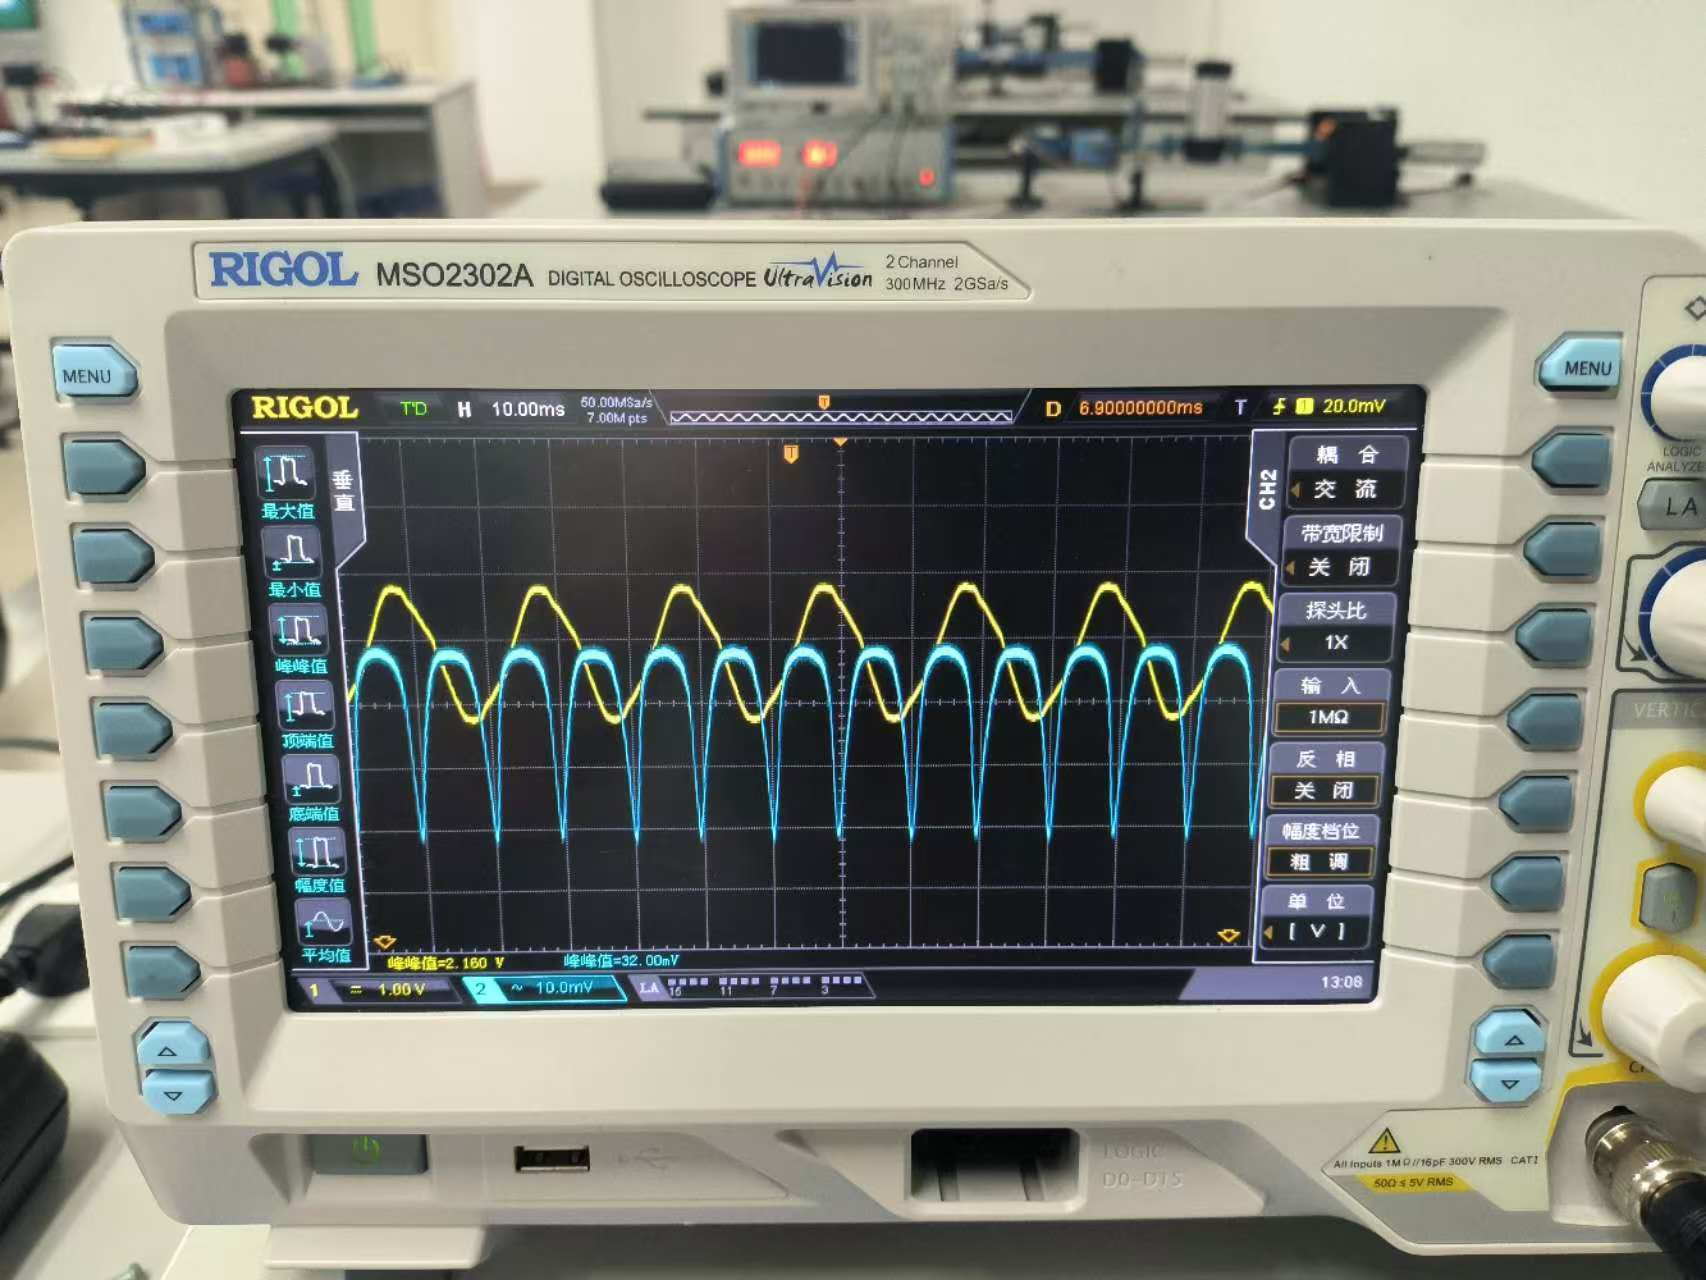
\includegraphics[width=0.5\textwidth]{D4-2-1.jpg}
			\caption{信号均匀出现的共振吸收信号}
			\label{fig:D4-2-1}
		\end{figure}




	\subsubsection{估测 DPPH 样品横向弛豫时间}

		由估算横向弛豫时间的公式$T_2 = \frac{2}{\gamma \Delta B}$可知,估算 $\Delta B$ 是关键。

		具体的实验步骤为:把带有移相器的扫场信号用线接入到示波器 CH1,检测输出的磁共振信号用线接入到示波器 CH2,将示波器切换到 X-Y 扫描模式,合成李萨如图。通过调节扫场相位,使两个共振峰重合。
		
		实验中主要使用两种方法估算$\Delta B$。
		\begin{itemize}
			\item \textbf{使用李萨如图直接拟合得到$\Delta B$}。
			
			\item \textbf{利用共振吸收信号拟合得到半高宽所对应的时间间隔,再根据扫场法原理间接得到半高宽}。
		\end{itemize}

		扫场磁场的测量方法:
		\begin{enumerate}
			\item 注意到,扫场磁场和励磁磁场\textbf{并不是一组线圈},所以不能通过实验一测得的电压和磁感应强度曲线和示波器CH1通道测量的电压得到扫场磁场的大小。
			\item 由扫场法原理,当励磁磁场满足共振吸收条件,此时再叠加扫场,每当扫场磁场为零时,会发生共振吸收,即在一个周期内发生两次共振吸收,记录下此时励磁电压的大小;此时将励磁磁场减小,使得扫场的极大值+励磁磁场满足共振吸收条件,即在一个周期内仅发生一次共振吸收,同样记录下此时励磁电压的大小。
			\item 两次励磁电压之差即对应扫场磁场的大小。
			\item 同时使用CH1通道的峰峰值建立扫场电压与扫场磁场大小的对应关系。
		\end{enumerate}

		测量得到的数据:
		\begin{itemize}
			\item 共振吸收信号为 10ms 时,励磁电压大小为:6.85V
			\item 共振吸收信号为 20ms 时,励磁电压大小为:5.80V
			\item 扫场电源的峰峰值:2.240V
		\end{itemize}





	\subsubsection{测量波导波长及微波波长}
		
		\begin{enumerate}
			\item 由实验原理可知,当谐振腔长度为半个波导波长的整数倍时,可观察到共振吸收信号。
			\item 改变谐振腔长度,当观察到共振吸收信号时,记录下此时谐振腔长度的读数(实验中可观察到两个共振吸收点)。
			\item 由这两个共振吸收点,可计算得到波导波长与微波波长。
			\item 测量到的两个共振吸收点为 $L_1 = 7.320 mm \quad L_2 = 30.663 mm$
		\end{enumerate}



		


	\subsection{实验过程中遇到的问题记录}

		\begin{enumerate}
			\item 高斯计调零时应当尽量远离磁场。
			\item DPPH样品应当放在谐振腔中驻波的波腹位置,实验中可尝试移动实验架,找到磁场最大的位置。
				
		\end{enumerate}



\clearpage
\subsection{实验数据记录}

	见\cref{fig:data}

	\begin{figure}[htbp]
		\centering
		% 第一行的两张图片
		\subfloat[原始数据1]
		{\includegraphics[width=0.3\textwidth]{D4-OriginalData-1.jpg}\label{fig:data1}}
		\quad
		\subfloat[原始数据2]
		{\includegraphics[width=0.3\textwidth]{D4-OriginalData-2.jpg}\label{fig:data2}}
		\newline
		% 第二行的两张图片
		\subfloat[原始数据3]
		{\includegraphics[width=0.3\textwidth]{D4-OriginalData-3.jpg}\label{fig:data3}}
		\quad
		\subfloat[原始数据4]
		{\includegraphics[width=0.3\textwidth]{D4-OriginalData-4.jpg}\label{fig:data4}}

		\caption{原始数据}
		\label{fig:data}
	\end{figure}
	



%\subsection{原始数据记录}


% \clearpage

	

\clearpage
\begin{table}
	\renewcommand\arraystretch{1.7}
	\begin{tabularx}{\textwidth}{|X|X|X|X|}
	\hline
	专业:& 物理学 &年级:& 2022级\\
	\hline
	姓名: & 戴鹏辉 \& 杨舒云 & 学号:& 22344016 \& 22344020\\
	\hline
    日期:& 2024/11/12 & 评分: &\\
	\hline
	\end{tabularx}
\end{table}

\section{D4-1 \quad 电子自旋共振实验 \quad\heiti 分析与讨论}

\subsection{实验数据分析}



	\subsubsection{确定励磁电压与磁感应强度关系曲线}

		对于\cref{tbl:D4-1-1}的数据,使用线性拟合,得到励磁电压与磁感应强度的大小关系:

		\begin{figure}[htbp]
			\centering
			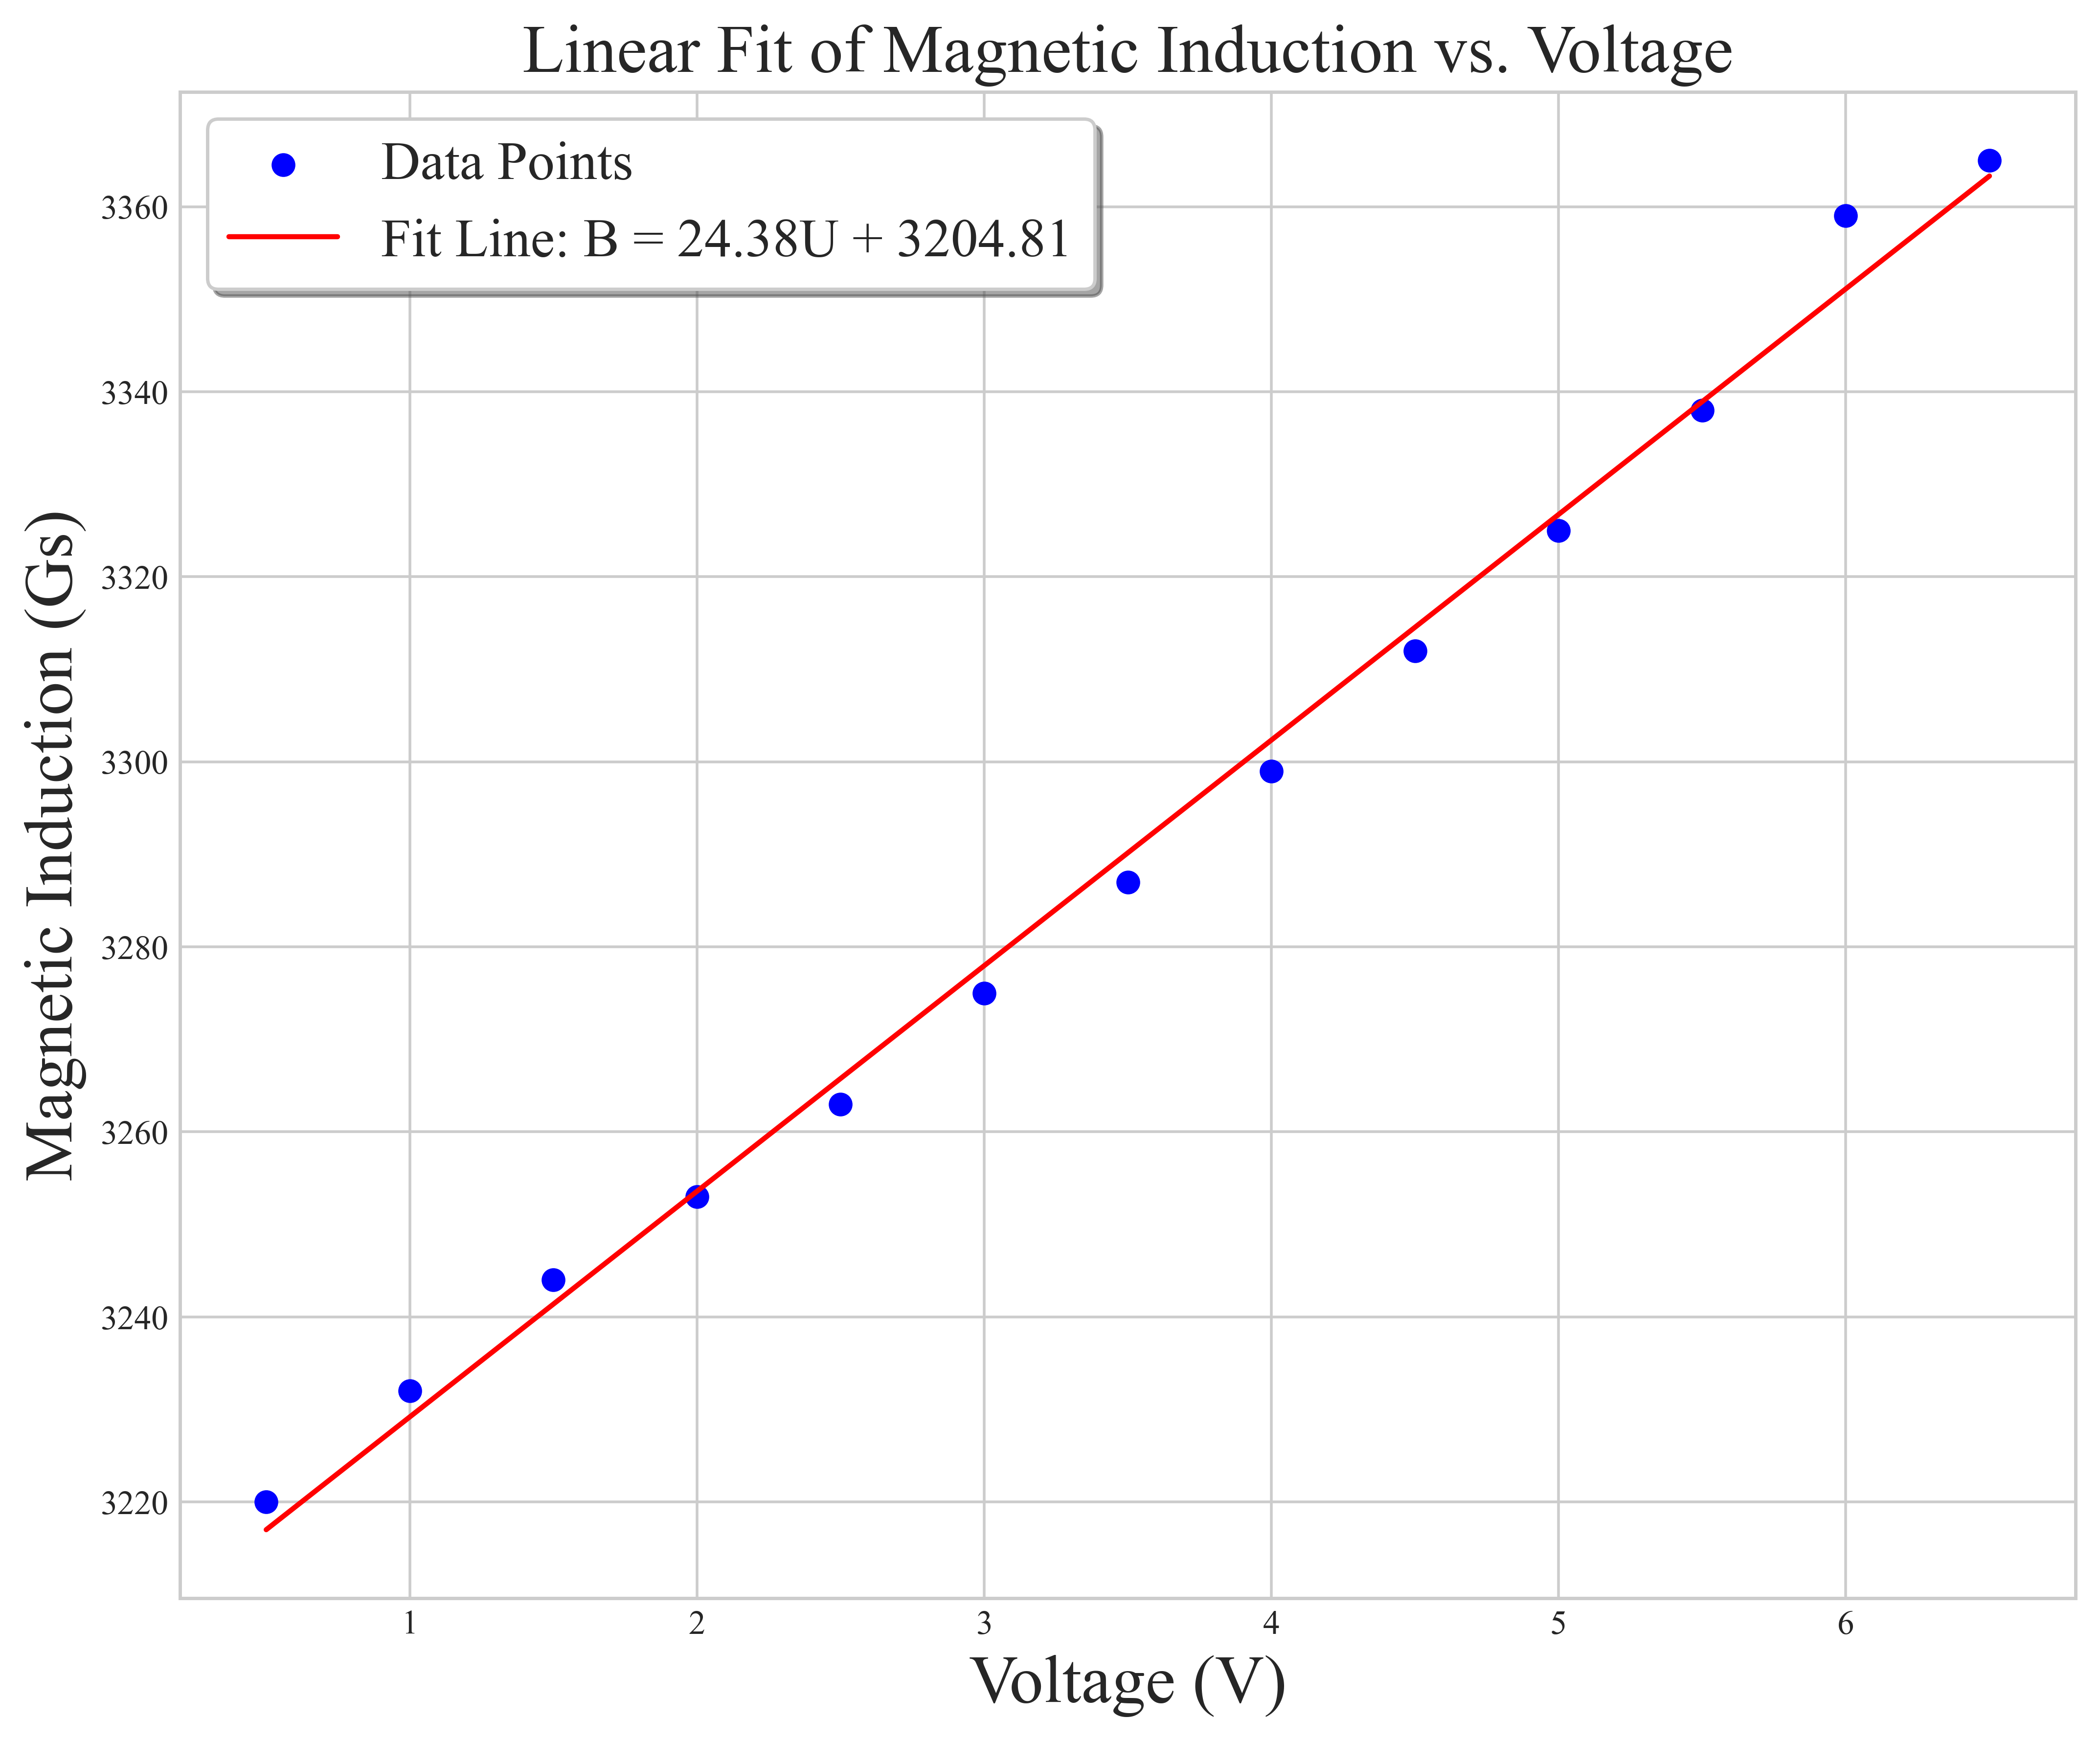
\includegraphics[width=0.7\textwidth]{D4-3-1.png}
			\caption{励磁电压与磁感应强度拟合拟合关系}
			\label{fig:D4-3-1}
		\end{figure}



	\subsubsection{观察磁共振信号并测定电子郎德因子}

		\begin{enumerate}
			\item 由\cref{tbl:D4-1-2}的数据,计算得到磁场大小,并代入公式计算朗德因子$g$:
				% \[
				% 	\omega = g \frac{\mu_B}{\hbar} B_0
				% \]
				\[
					g = \frac{\mu_B \cdot B_0}{f \cdot h}
				\]

			\item 根据测量结果,计算得到的朗德因子结果为 $g = 1.9906$。
			
			\item 下面进行误差分析:
			
				朗德因子的标准差由下面公式计算得到:
				\begin{align*}
					\sigma_g = \sqrt{(\frac{\partial g}{\partial B_0} \sigma_{B_0})^2 + (\frac{\partial g}{\partial f} \sigma_f)^2} = 0.00128
				\end{align*}
				
				相对不确定度为:
				\[
					\eta_1 = \frac{\sigma_g}{g} \times 100 \% = 0.1279 \%
				\]

				测量值与标准值的相对误差为:
				\[
					\eta_2 = \frac{g - g_0}{g_0} \times 100 \% = -0.6215 \%
				\]
			
		\end{enumerate}

		可见,相对不确定度为 $0.1279 \%$,说明测量结果比较精确。但是与标准值比较可以发现,测量结果偏小。由朗德因子计算公式可知,可能的原因为测量的磁感应强度偏小、或测量的微波频率偏大。

		\begin{itemize}
			\item 在实验中,磁感应强度由高斯计来测定。如果高斯计的校准存在偏差(即系统误差),可能导致磁场强度测量结果有较大误差。虽然在实验一测量励磁电压与磁感应强度关系曲线之前,已经对高斯计进行了校准,可能是因为在校准时没有完全屏蔽磁场,或者是高斯计自身有个系统性的偏差。
			\item 实验中我们使用吸收式频率计测量频率,具体是观察示波器波形是否发生跳动。由于旋转频率计是从示数小向示数大的方向旋转,且人的动作有延迟,所以在观察到波形跳动后旋转才停止,可能导致频率计测量频率偏大。
		\end{itemize}

		% 比标准值偏小?






	\subsubsection{估测 DPPH 样品横向弛豫时间}
		
		首先考虑扫场磁场的测量:
		\begin{enumerate}
			\item 扫场磁场的大小:
				\[
					B' = 24.38 \times (6.85 - 5.80) \mathrm{Gs} = 25.60 \mathrm{Gs}
				\]

			\item 单位扫场电源电压对应扫场磁场大小:
				\[
					k = 2 \times \frac{B'}{V_{pp}} = 2 \times \frac{25.60}{2.240} \mathrm{Gs/V} = 23.21 \mathrm{Gs/V}
				\]
		\end{enumerate}



		\vspace{1cm}



		对于示波器导出的数据,我们将按照如下的步骤进行分析与处理:
		\begin{enumerate}
			\item 将数据分为多个周期并求平均,得到一个周期内的平均值,以减小噪声并提高数据的平滑度。
			\item 由于导出的数据中,时间序列的数据间隔为单位时间,而不是秒,所以需要根据采样率定义周期。周期长度 $T_{x1}$ 和 $T_{y1}$ 被设定为 400,以适应数据的周期性结构。多个周期平均后的数据便于后续滤波和拟合。
			\item 使用 Savitzky-Golay 滤波器 对平均化后的 X 和 Y 数据进行平滑处理,以去除高频噪声。Savitzky-Golay 滤波器可以有效保持信号的趋势,并在平滑的同时尽量不改变信号的主要形状。
			\item 为了进一步分析和绘制李萨如图,将平滑后的 X 和 Y 数据从索引 50 到 200 截取。这样的截取确保选择的片段位于信号稳定且噪声较小的区域,减少边界效应对拟合结果的干扰。
			\item 使用 Lorentzian 函数 对李萨如图数据进行拟合。Lorentzian 是常见的共振曲线拟合函数,适用于 ESR 信号分析。拟合得到的参数包括中心位置 $x_0$、全宽半高(FWHM)$\Gamma$、幅值 $A$ 和基线 $y_0$ 。
				\[
					f(x) = y_0 - \frac{A}{1 + (\frac{x - x_0}{\Gamma / 2})^2}
				\]
			\item 时序图的拟合分两种情况进行,分别是“平均时序图”和“普通时序图”。与李萨如图类似,时序图也使用 Lorentzian 拟合。
				\begin{itemize}
					\item 平均时序图拟合:对 Y 数据重新按 200 个数据点为周期进行平均,获得平滑后的时序图数据并进行 Lorentzian 拟合。拟合后的 FWHM 用于计算弛豫时间。
					\item 普通时序图拟合:直接对选定的 Y 数据片段拟合,得到另一组 FWHM 参数,并用于计算弛豫时间。
				\end{itemize}
		\end{enumerate}

		% 将示波器的X-Y-t数据导出后,进行进一步的分析与处理。
		% \begin{enumerate}
		% 	\item 首先进行周期平均化,绘制李萨如图和时序图
			
		% 		% 如\cref{fig:D4-3-2}、\cref{fig:D4-3-3}:
		% 		% \begin{figure}[htbp]
		% 		% 	\centering
		% 		% 	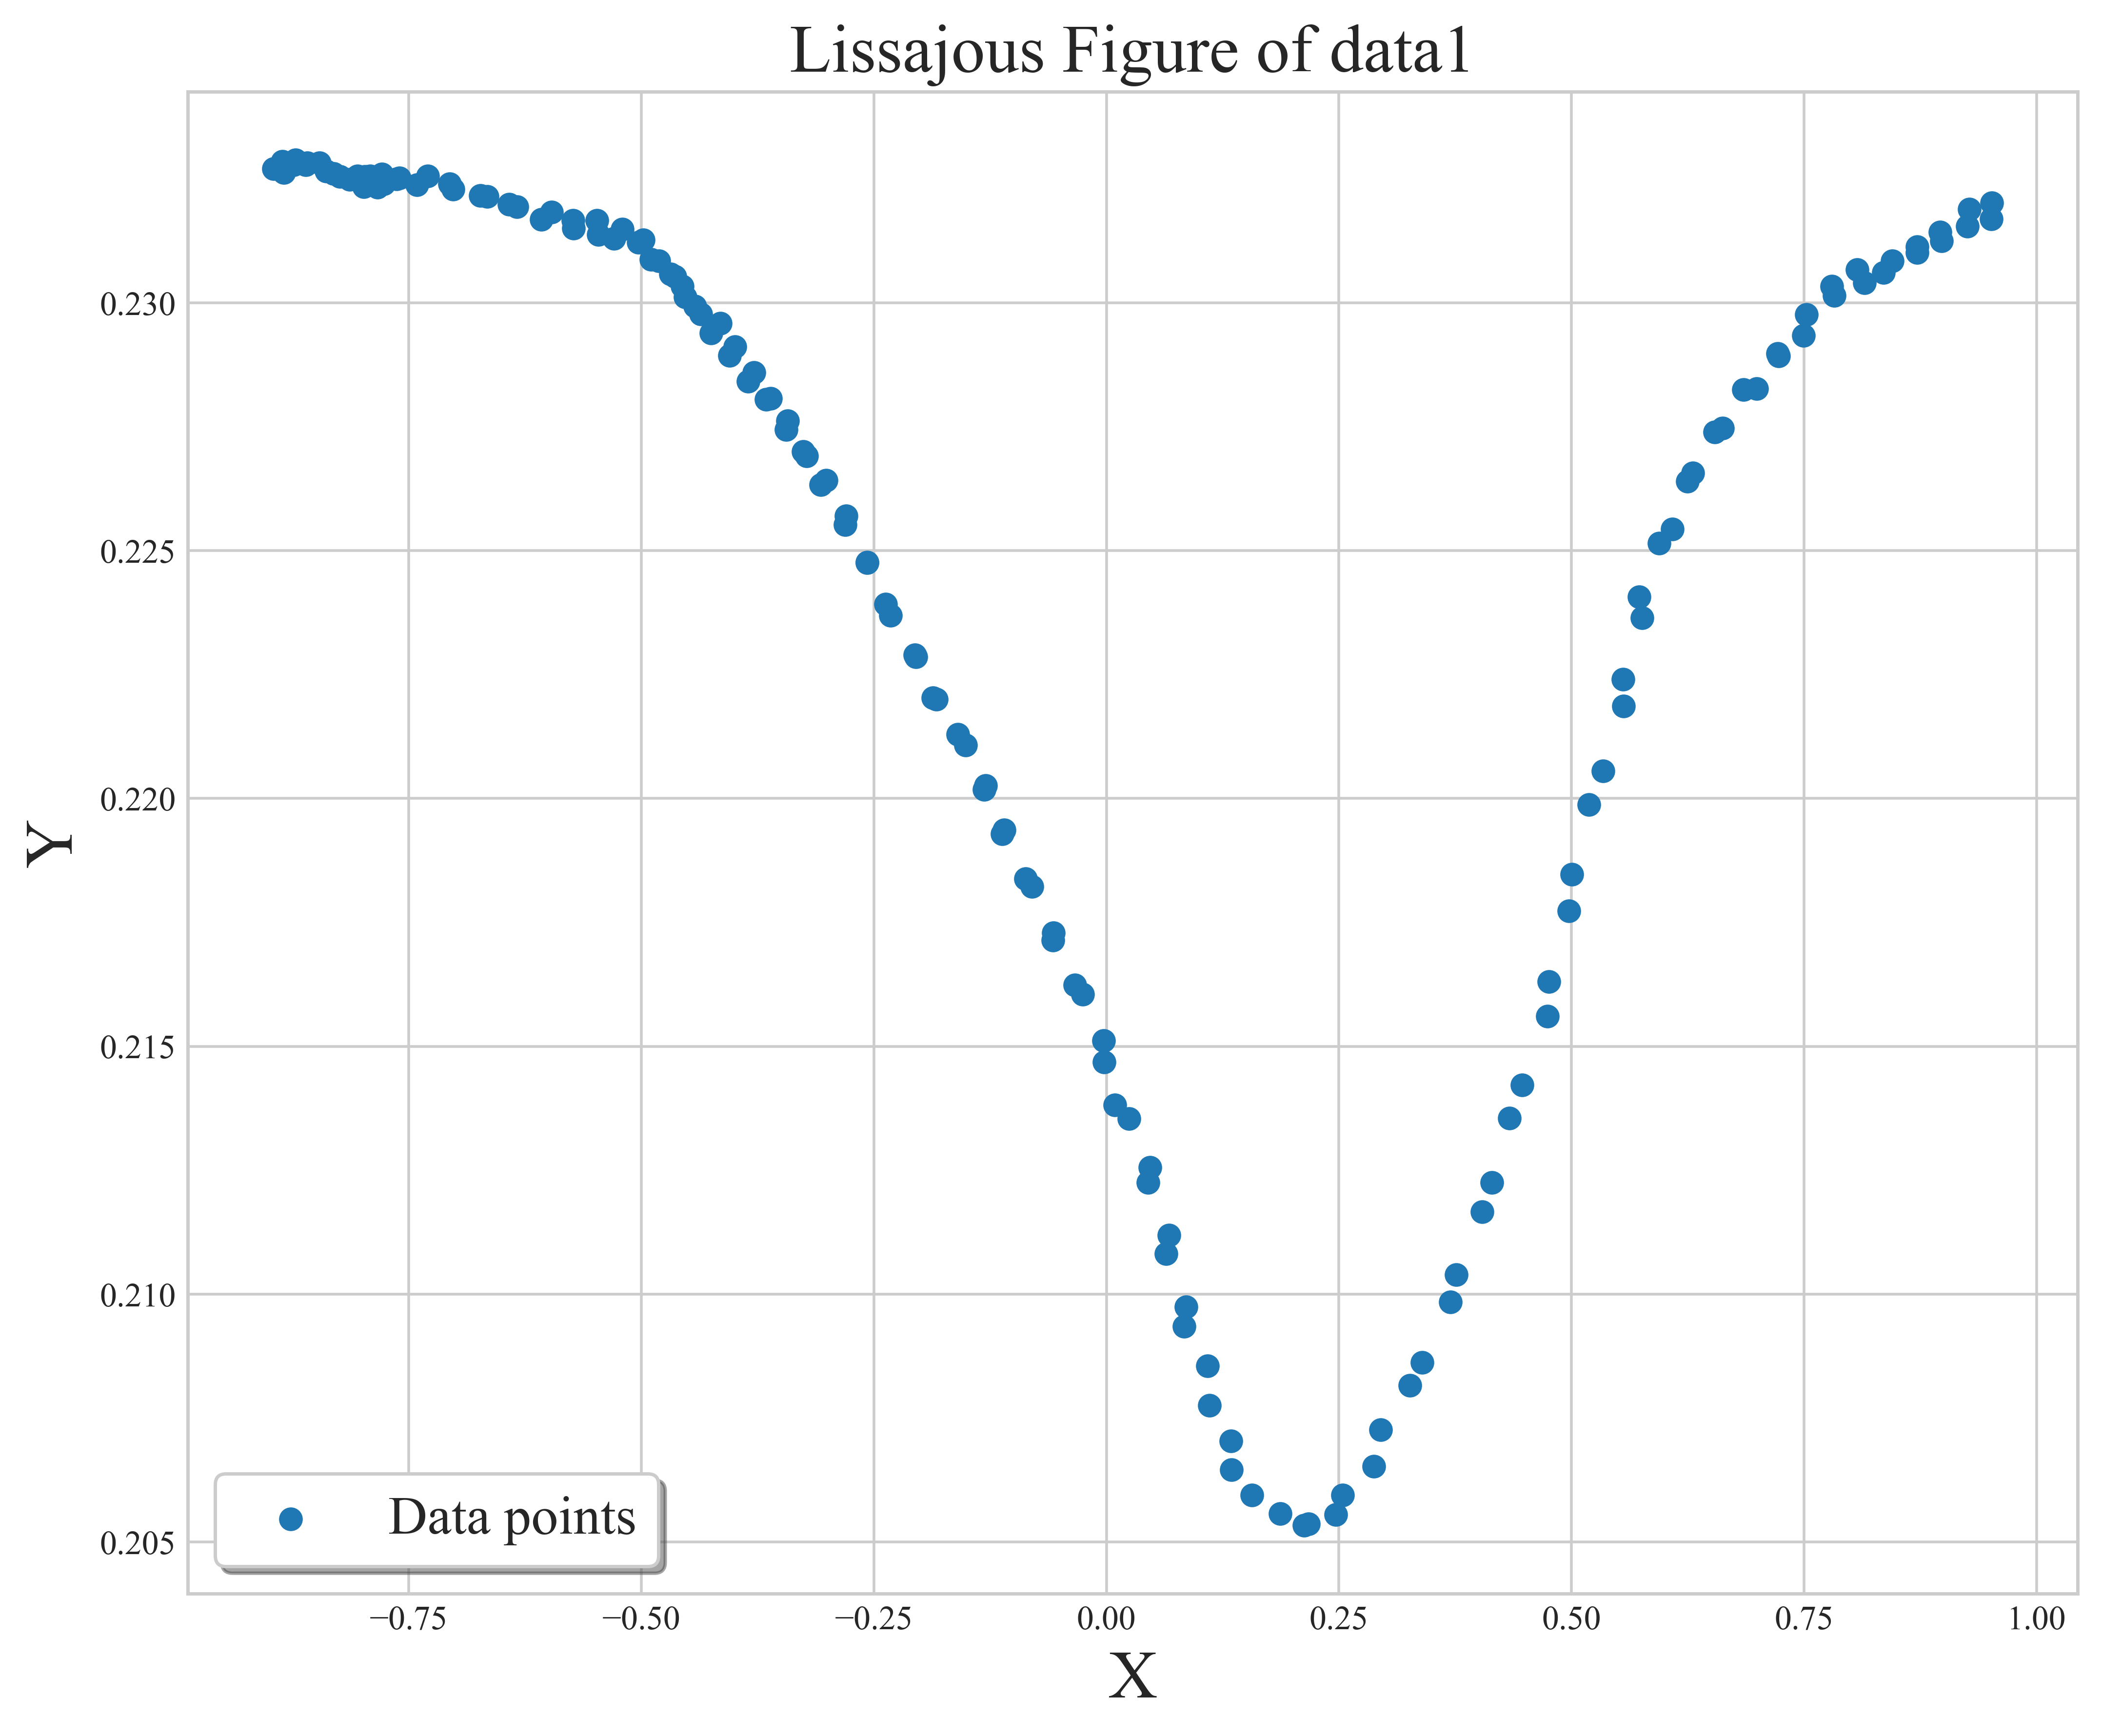
\includegraphics[width=0.7\textwidth]{D4-3-2.png}
		% 		% 	\caption{李萨如图}
		% 		% 	\label{fig:D4-3-2}
		% 		% \end{figure}
		% 		% \begin{figure}[htbp]
		% 		% 	\centering
		% 		% 	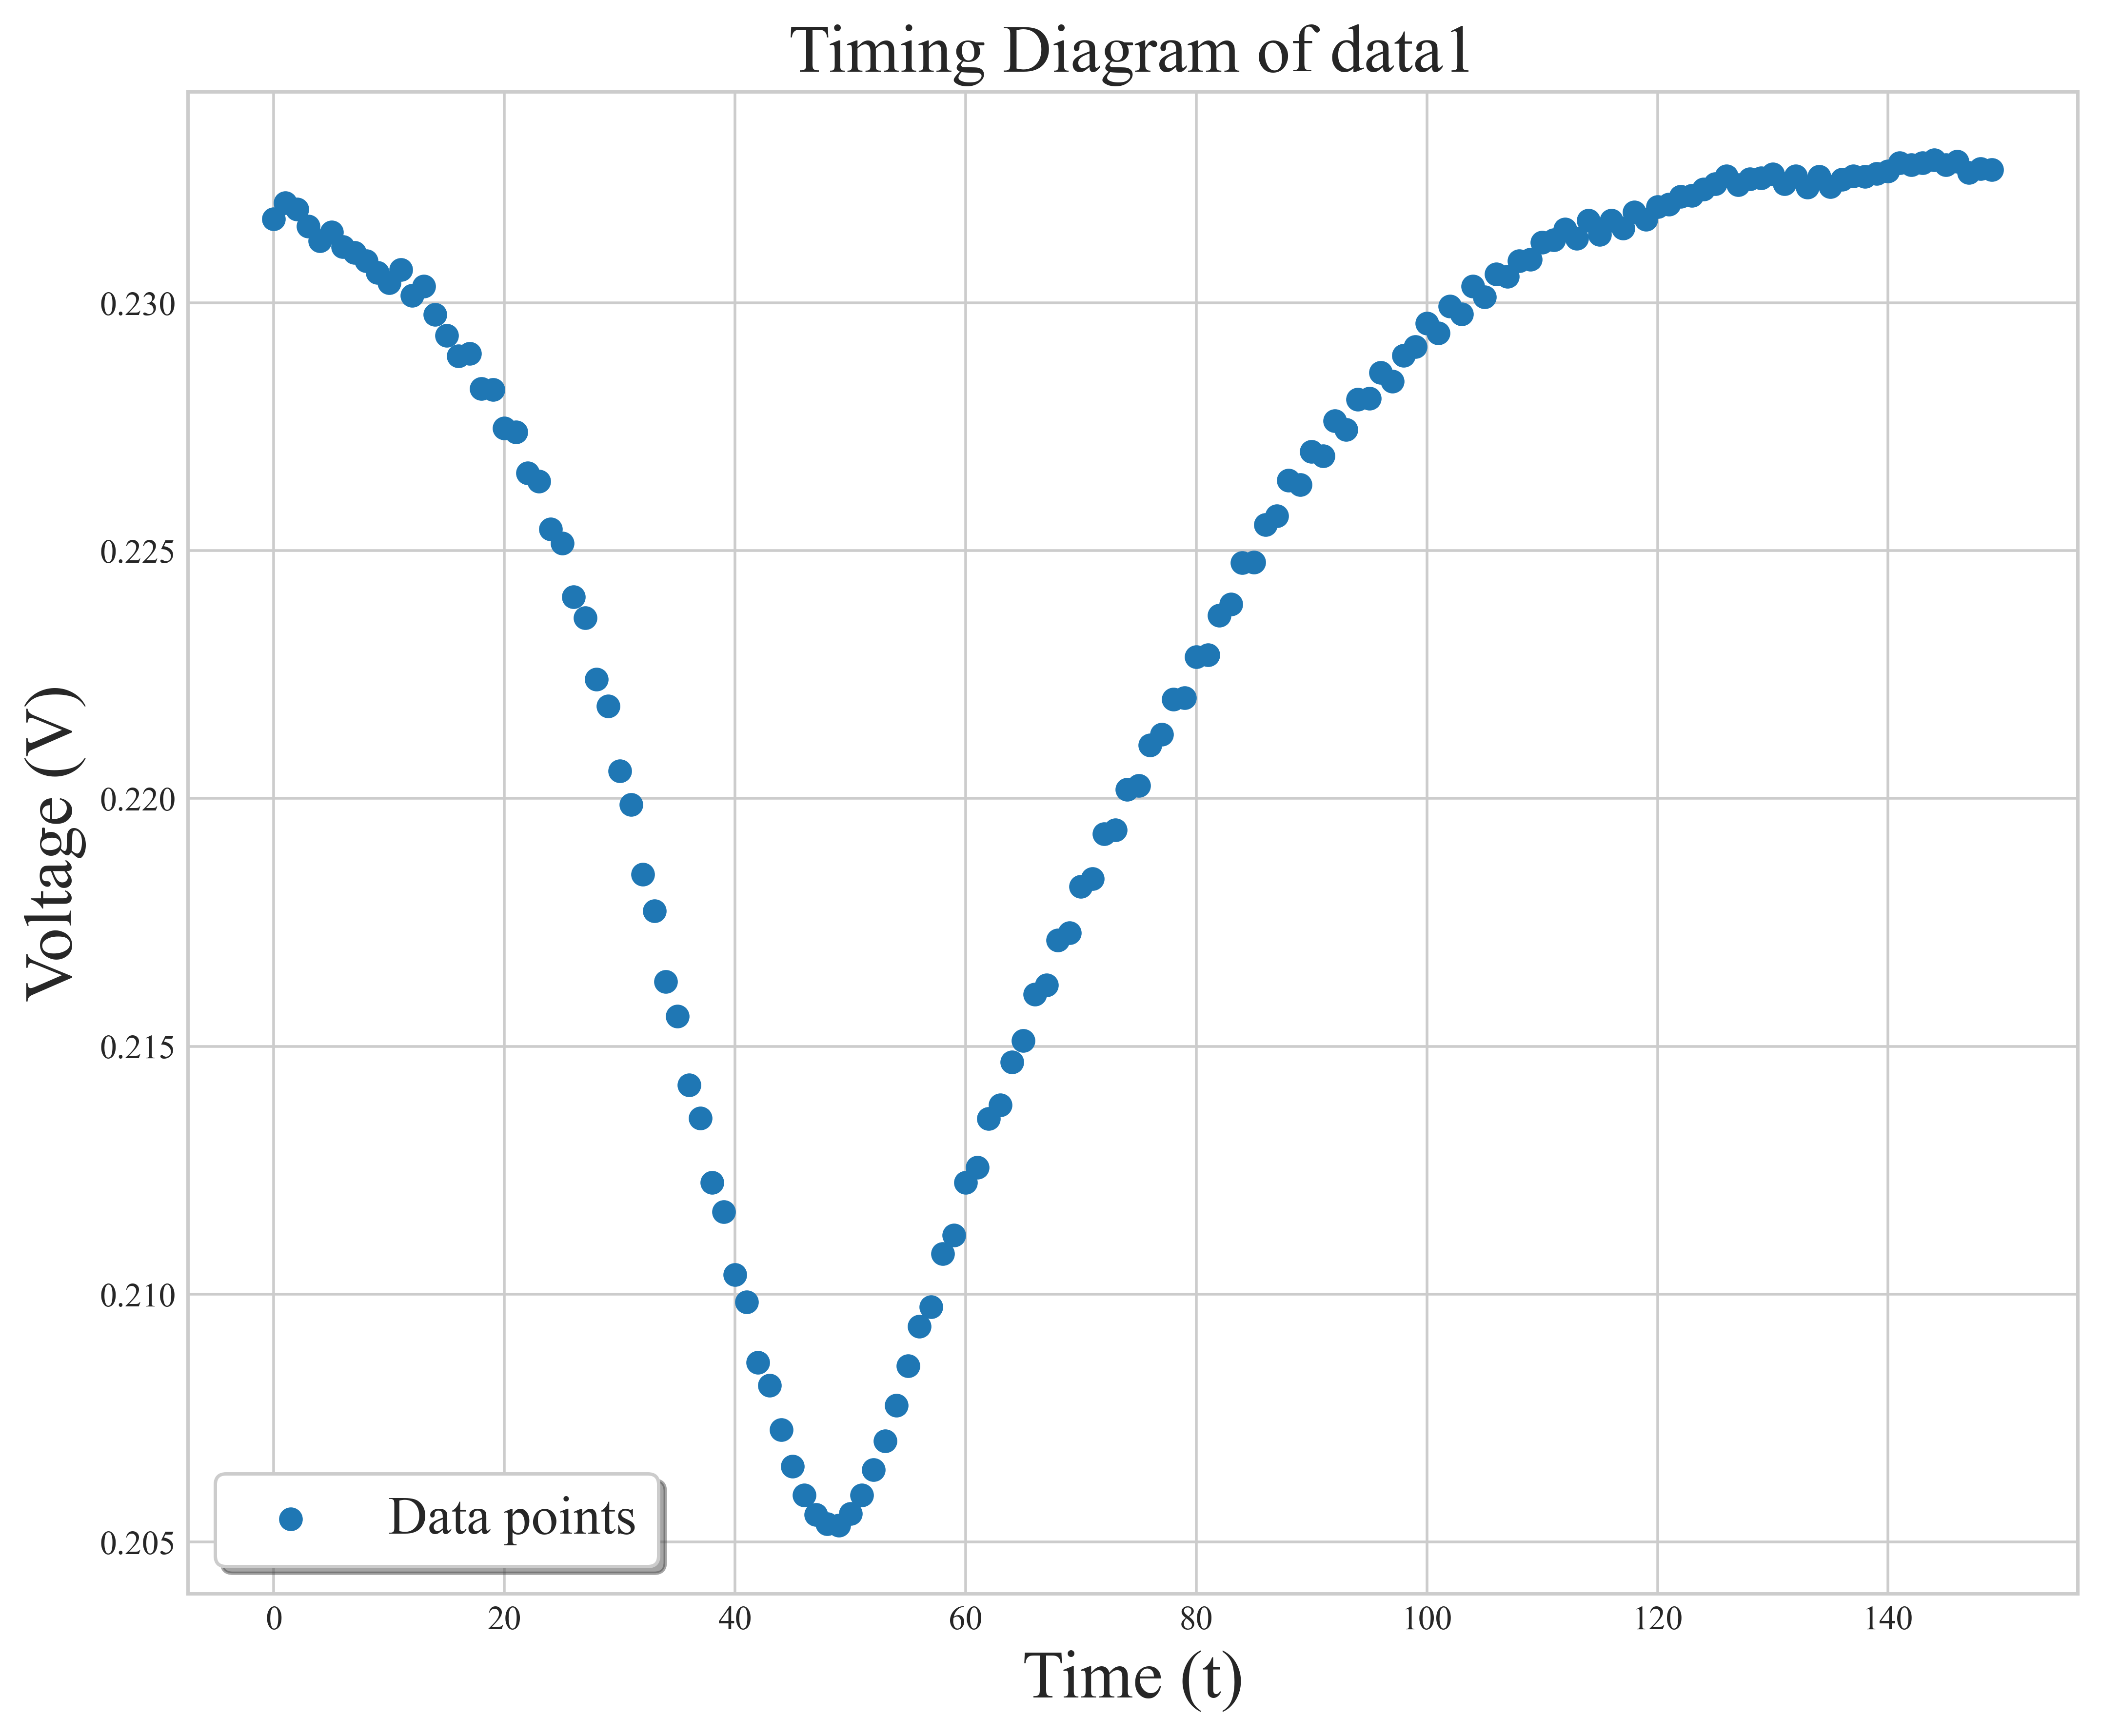
\includegraphics[width=0.7\textwidth]{D4-3-3.png}
		% 		% 	\caption{时序图}
		% 		% 	\label{fig:D4-3-3}
		% 		% \end{figure}

		% \end{enumerate}


		\begin{itemize}
			\item 首先考虑拟合李萨如图的方法:

				% 使用洛伦兹曲线拟合:
				% \[
				% 	f(x) = y_0 - \frac{A}{1 + (\frac{x - x_0}{\Gamma / 2})^2}
				% \]

				得到的拟合结果如\cref{fig:D4-3-4}:
				\begin{figure}[htbp]
					\centering
					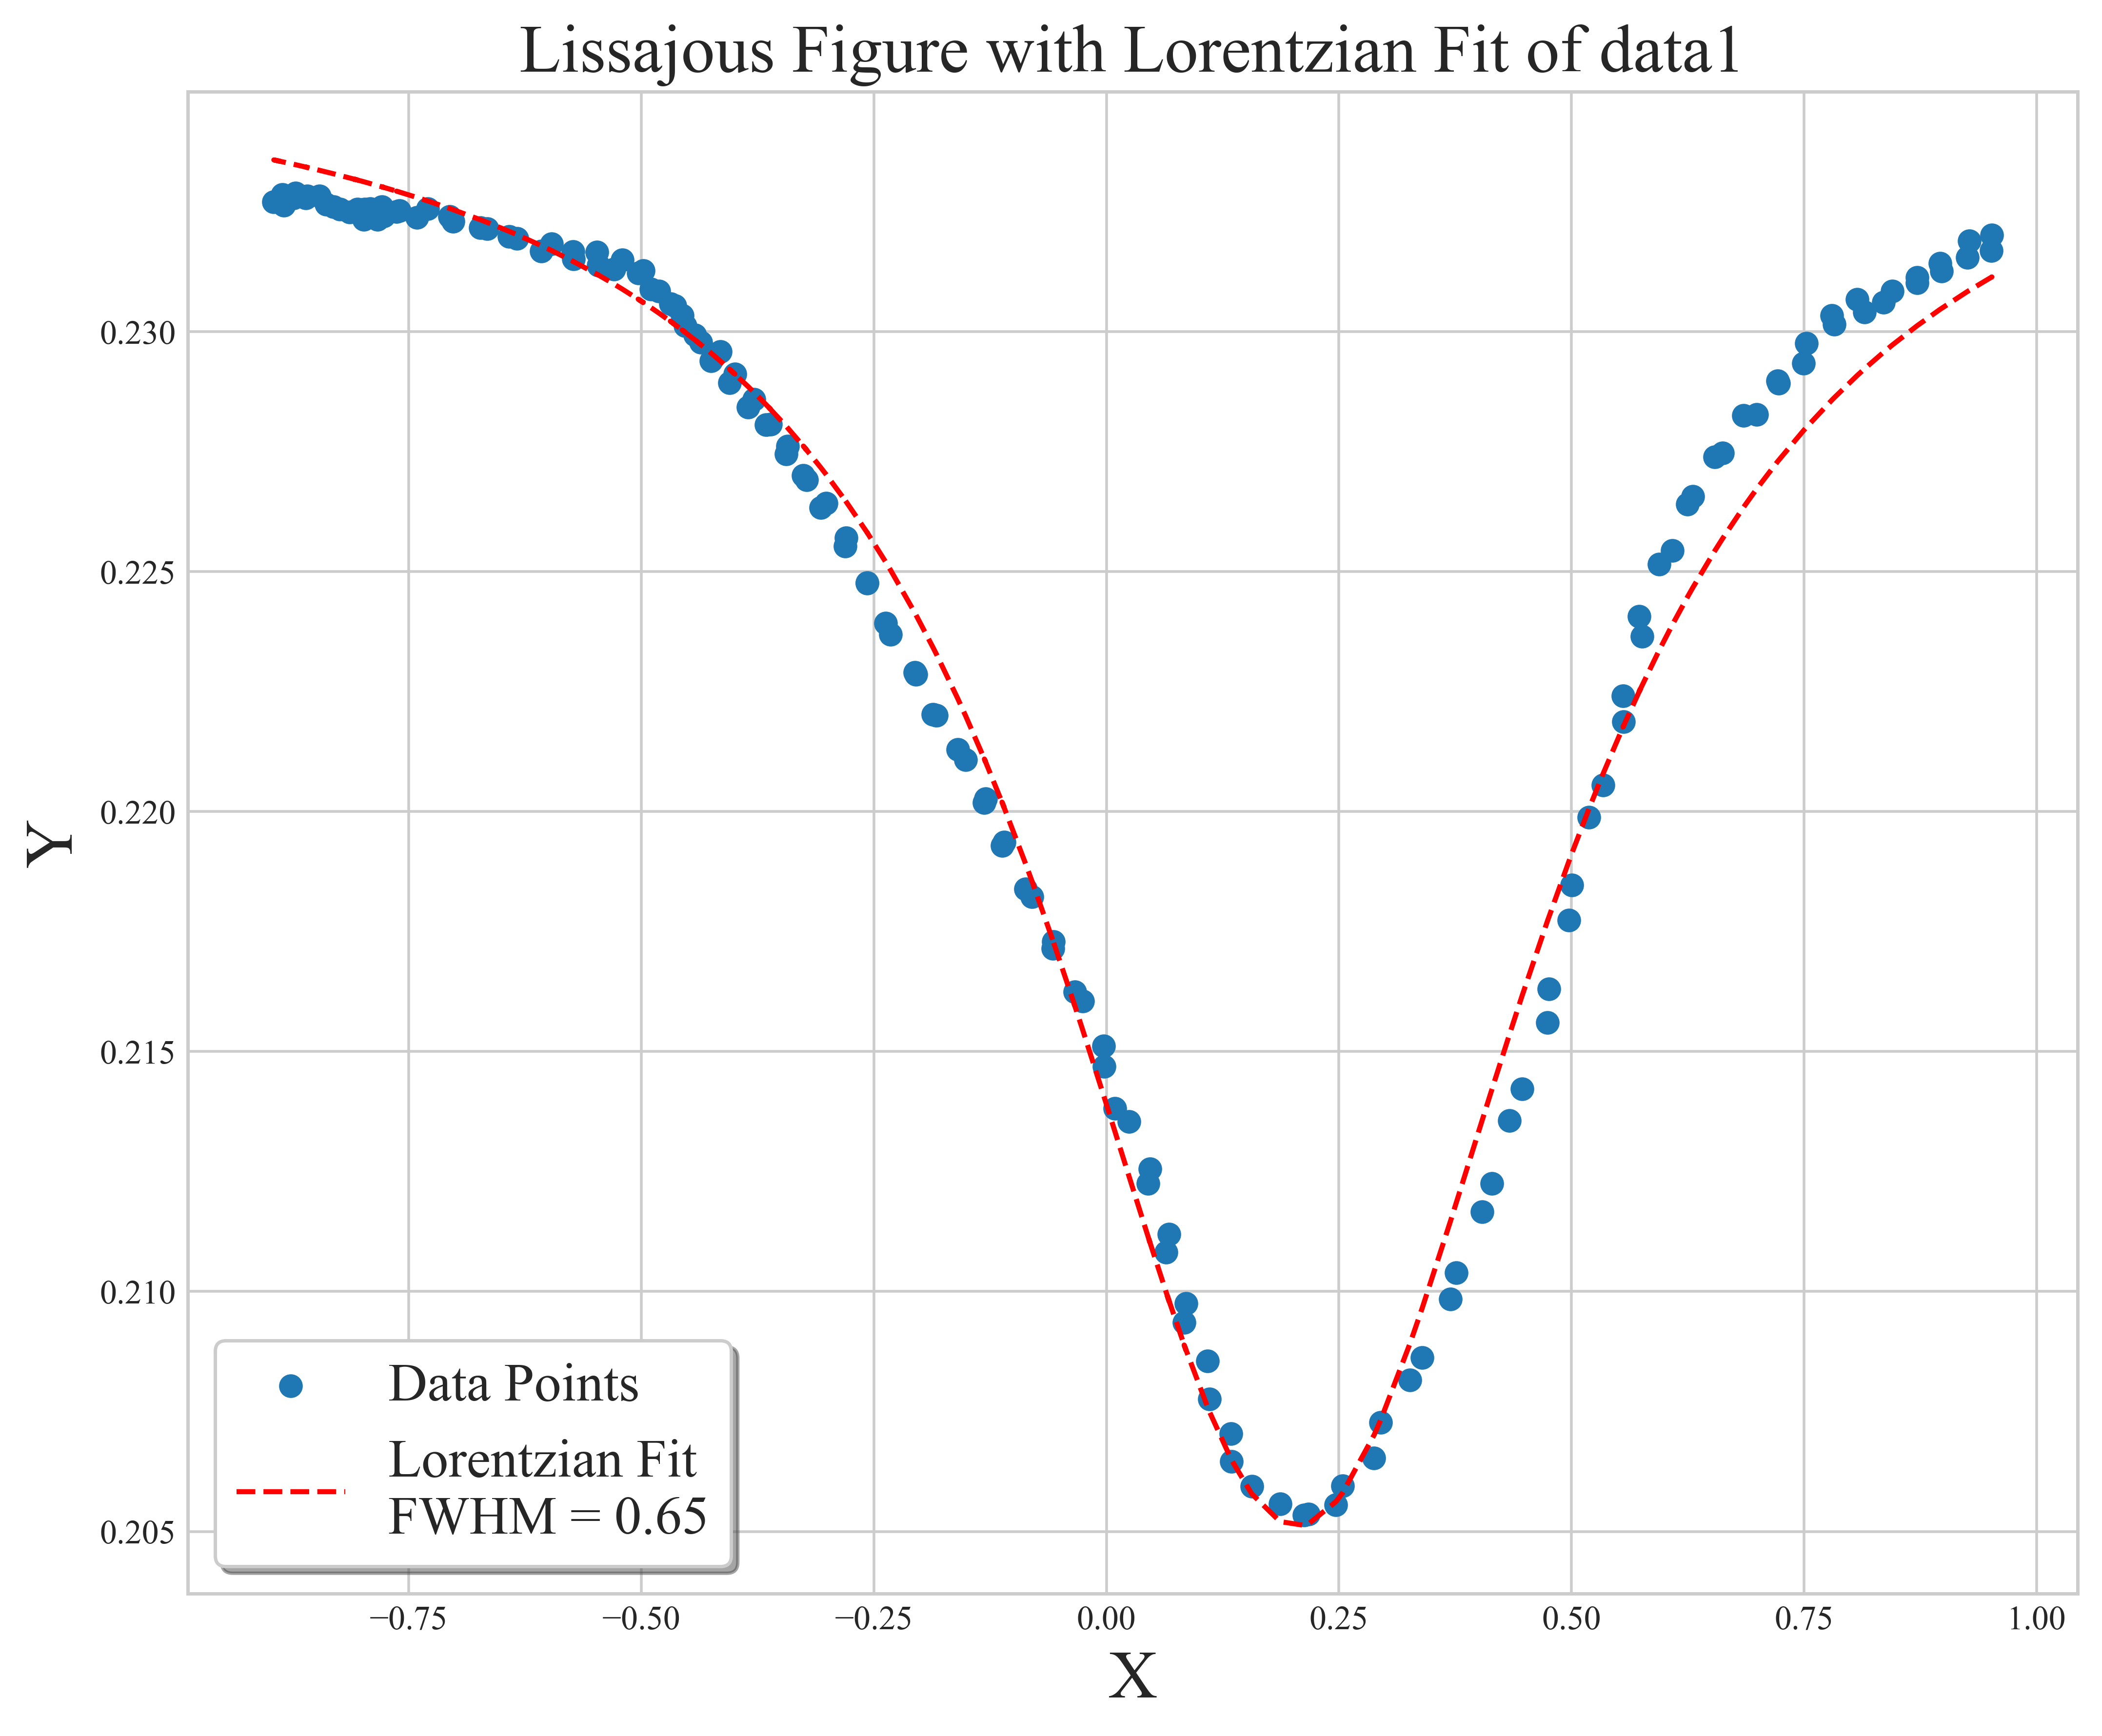
\includegraphics[width=0.7\textwidth]{D4-3-4.png}
					\caption{洛伦兹峰拟合李萨如图}
					\label{fig:D4-3-4}
				\end{figure}

				得到曲线的全高半宽为 0.65。于是得到$\Delta B = k \cdot 0.65  = 0.0008566 \mathrm{T}$
				\[
					\Rightarrow T_2 = \frac{2}{\gamma \Delta B} = 7.2838 \mathrm{ns}
				\]


			\item 再考虑拟合时序图的方法:
				
				考虑如下方式计算 $\Delta B$:
				\begin{align*}
					\Delta B = B' \sin \omega t_2 - B' \sin \omega t_1 = 2 B' \cos\omega\frac{t_2 + t_1}{2} \cdot \sin\omega\frac{t_2 - t_1}{2} = 2 B' \sin\frac{\omega \Delta t}{2}
				\end{align*}
				分别使用"平均时序图拟合"和"时序图拟合"的方法,对其拟合,得到结果如\cref{fig:D4-3-5}、\cref{fig:D4-3-6}(其中横轴为单位时间长度):

				分别得到全高半宽为 “53.62” 和 “42.19”,分别对应
				\begin{align*}
					\Delta t_1 = \frac{53.62 \times 10^{-3}}{200} = 0.00268 s \\
					\Delta t_2 = \frac{42.19 \times 10^{-3}}{200} = 0.00211 s
				\end{align*}

				分别计算横向弛豫时间$T_2$,结果为:
				\begin{enumerate}
					\item 平均时序图拟合得到弛豫时间 $T_2$ = 5.4265 ns
					\item 时序图拟合得到弛豫时间 $T_2$ = 6.8187 ns
				\end{enumerate}

				\begin{figure}[htbp]
					\centering
					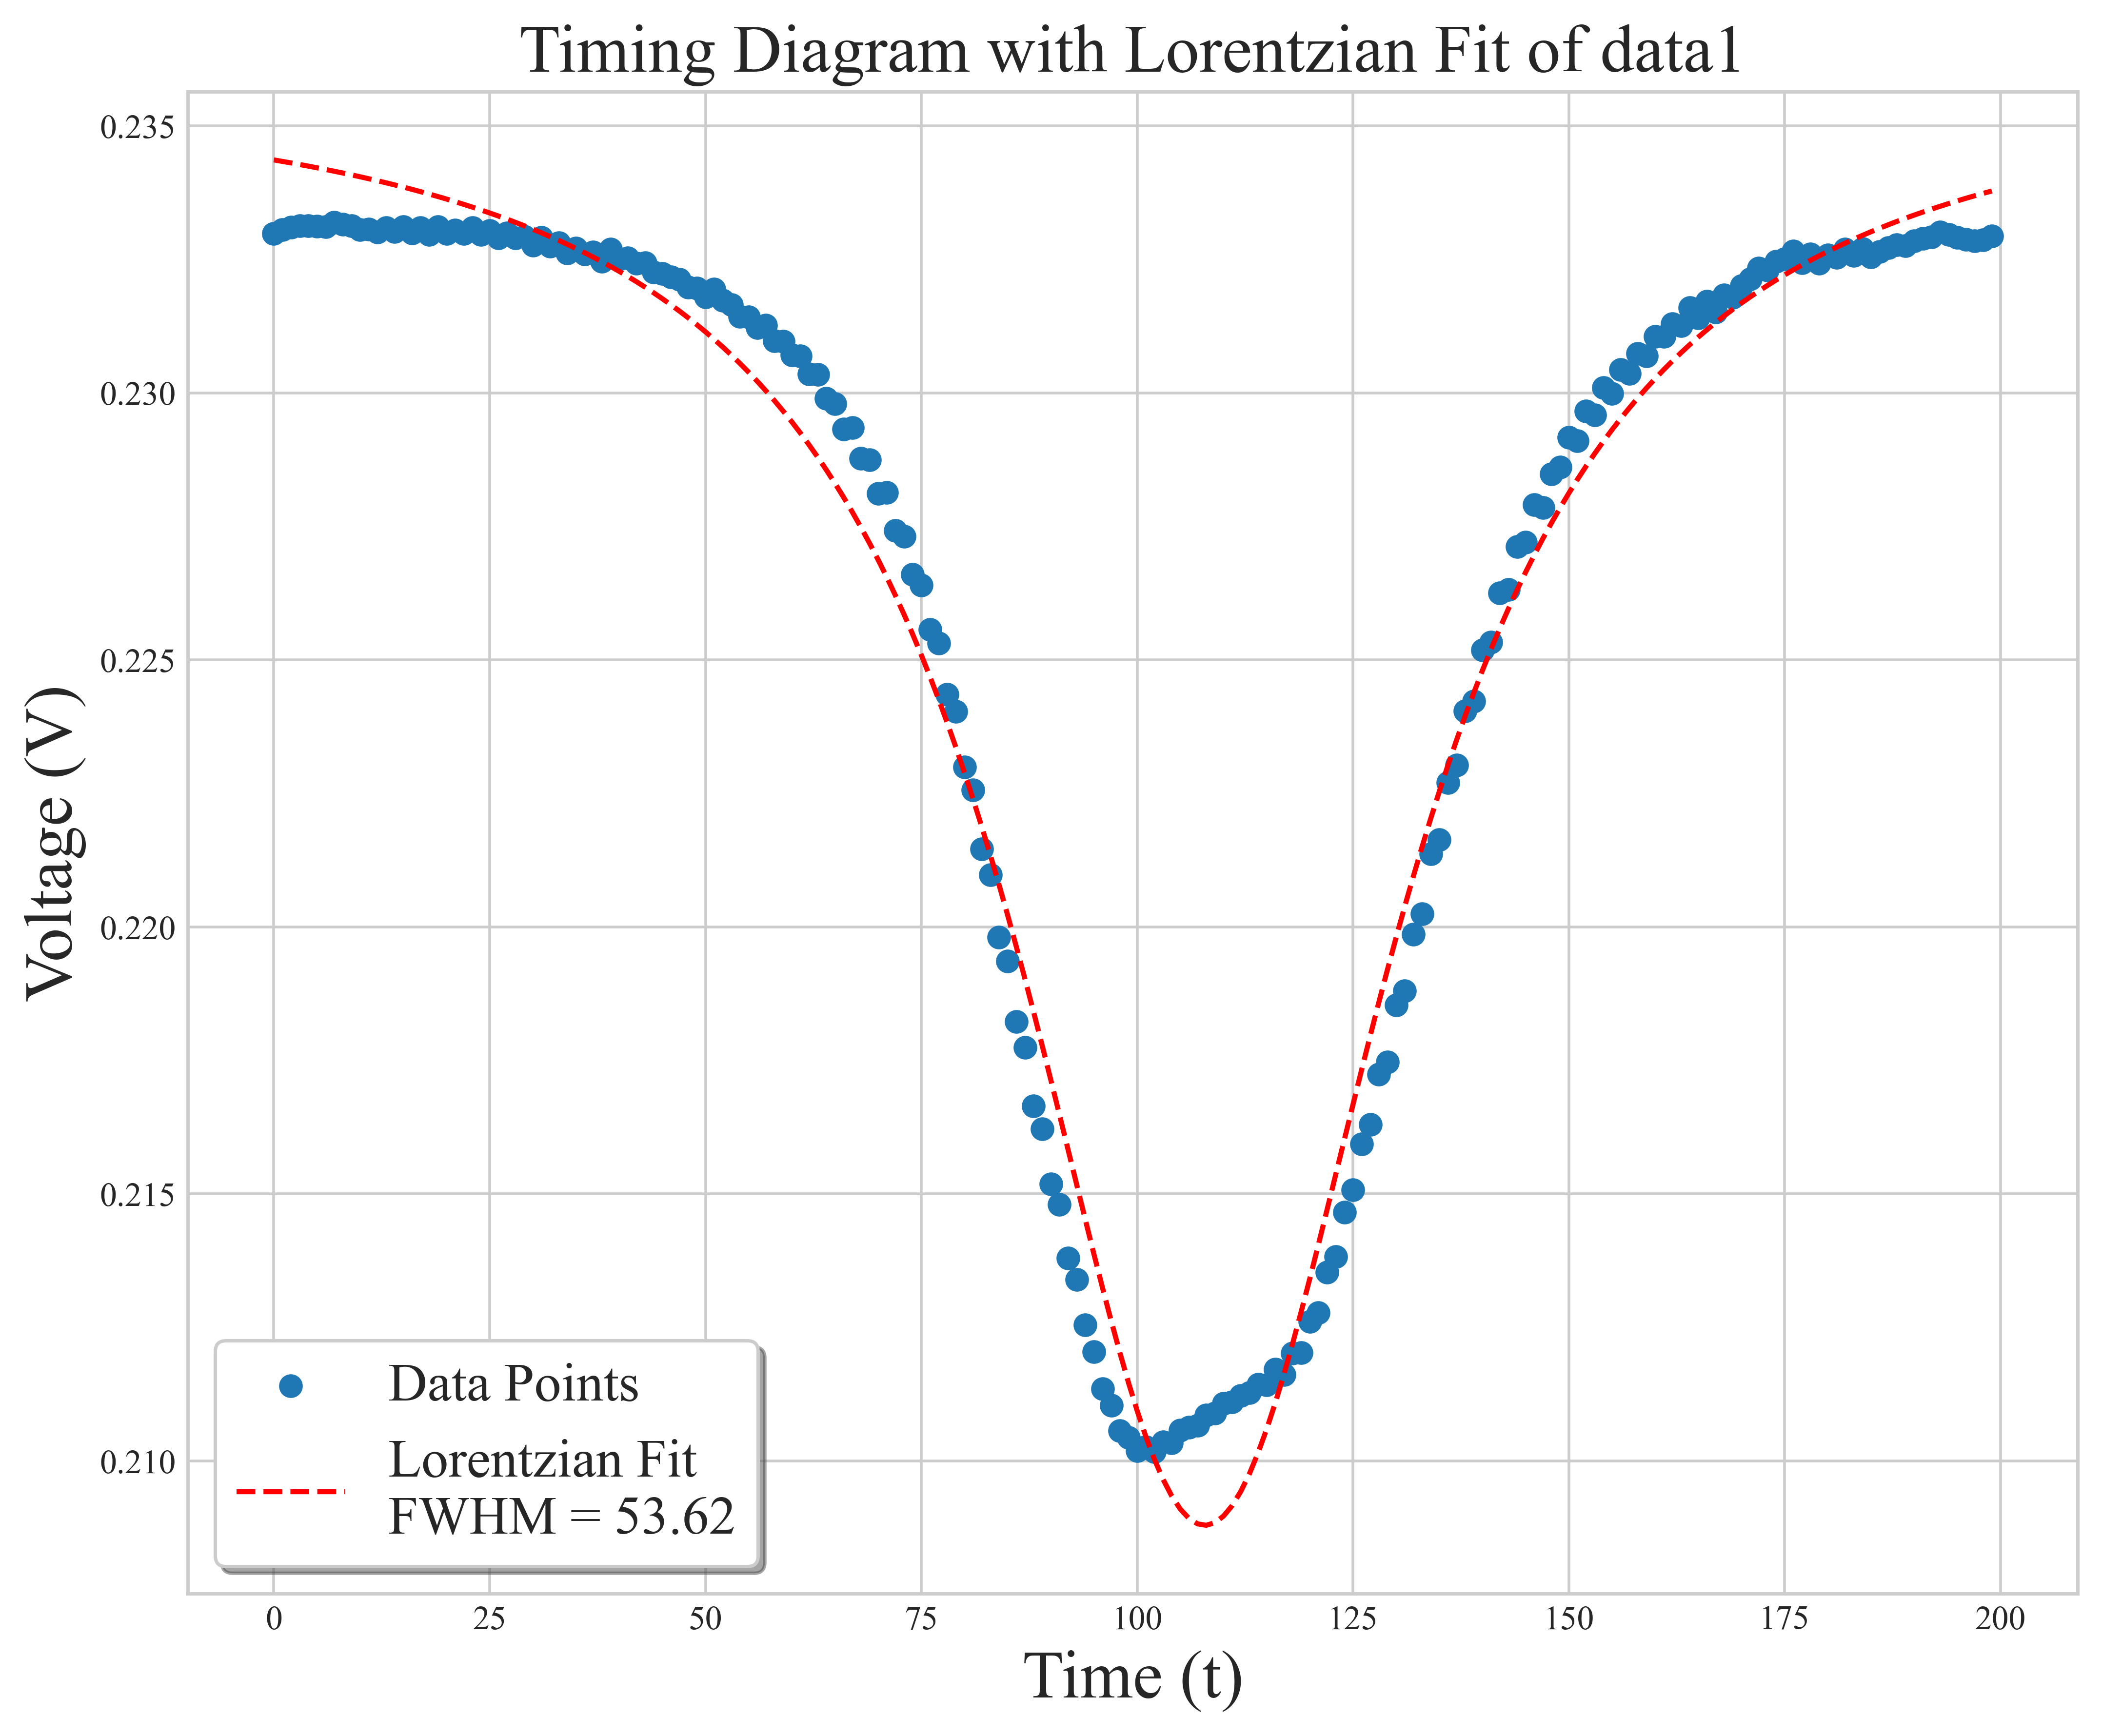
\includegraphics[width=0.7\textwidth]{D4-3-5.png}
					\caption{data1平均时序图拟合}
					\label{fig:D4-3-5}
				\end{figure}
				\begin{figure}[htbp]
					\centering
					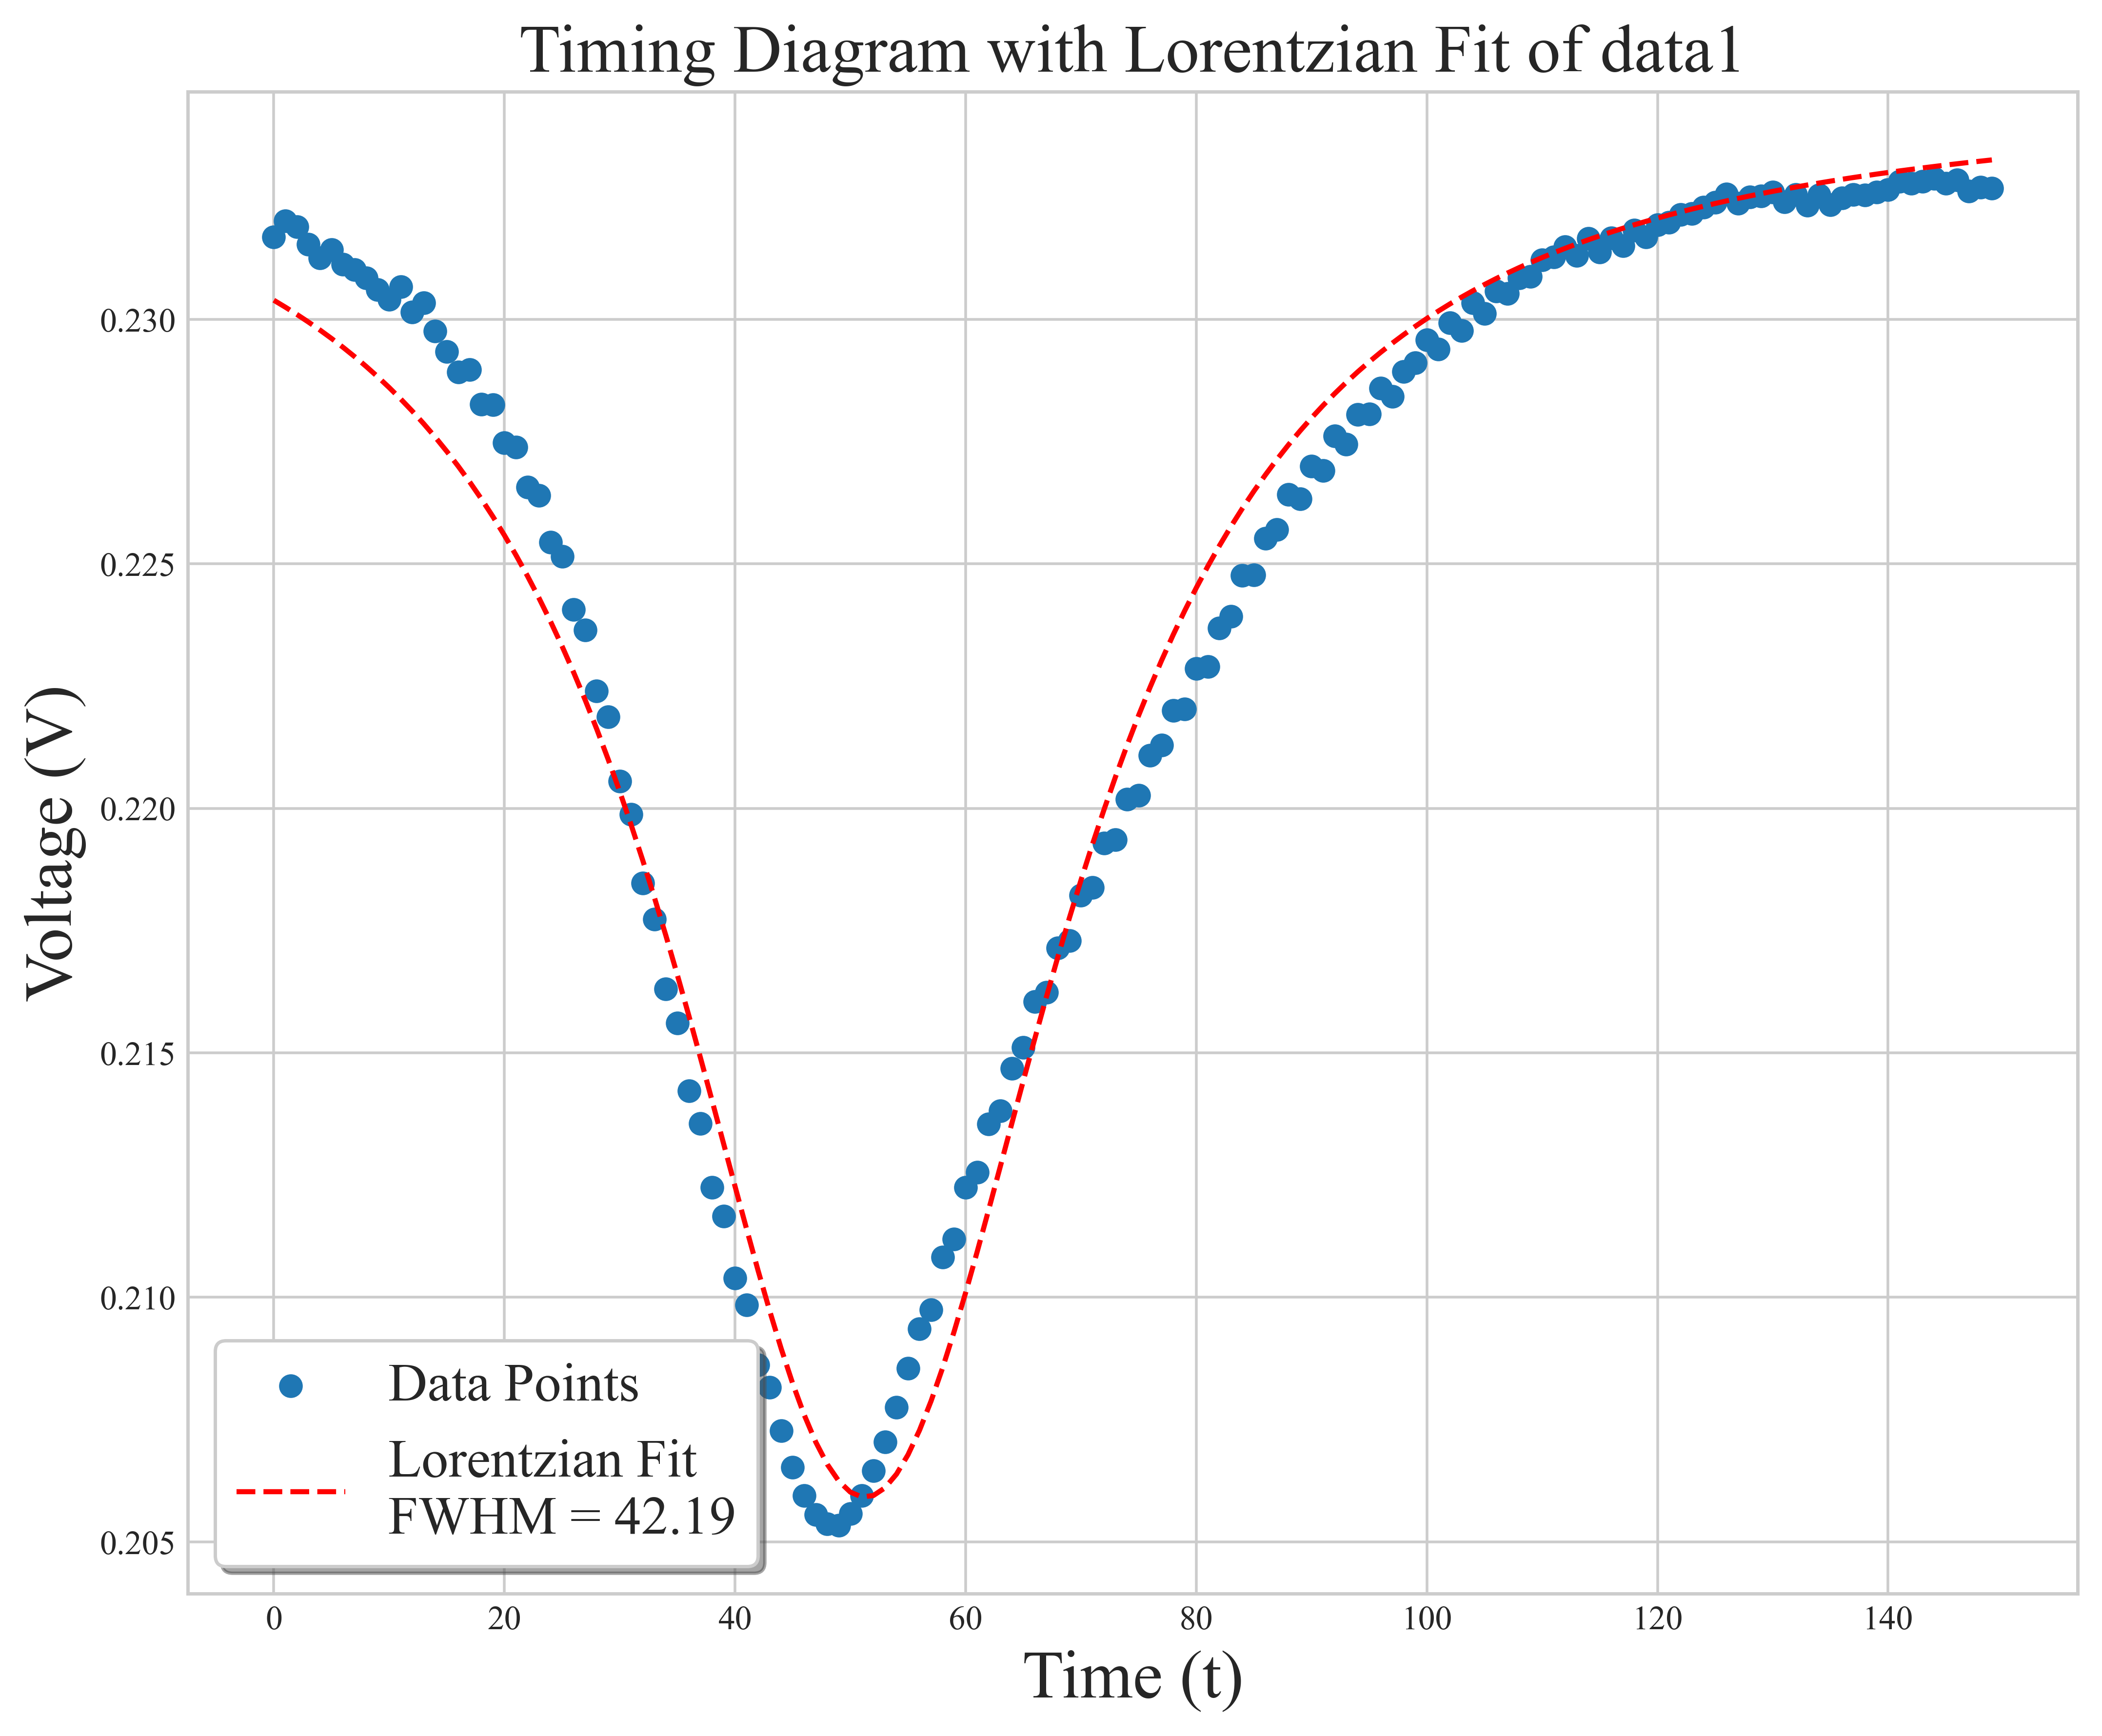
\includegraphics[width=0.7\textwidth]{D4-3-6.png}
					\caption{data1时序图拟合}
					\label{fig:D4-3-6}
				\end{figure}

				
		\end{itemize}


		按照上述方法,对第二组数据 data2 进行同样的分析处理,结果如\cref{fig:D4-3-7}、\cref{fig:D4-3-8}:
		\begin{figure}[htbp]
			\centering
			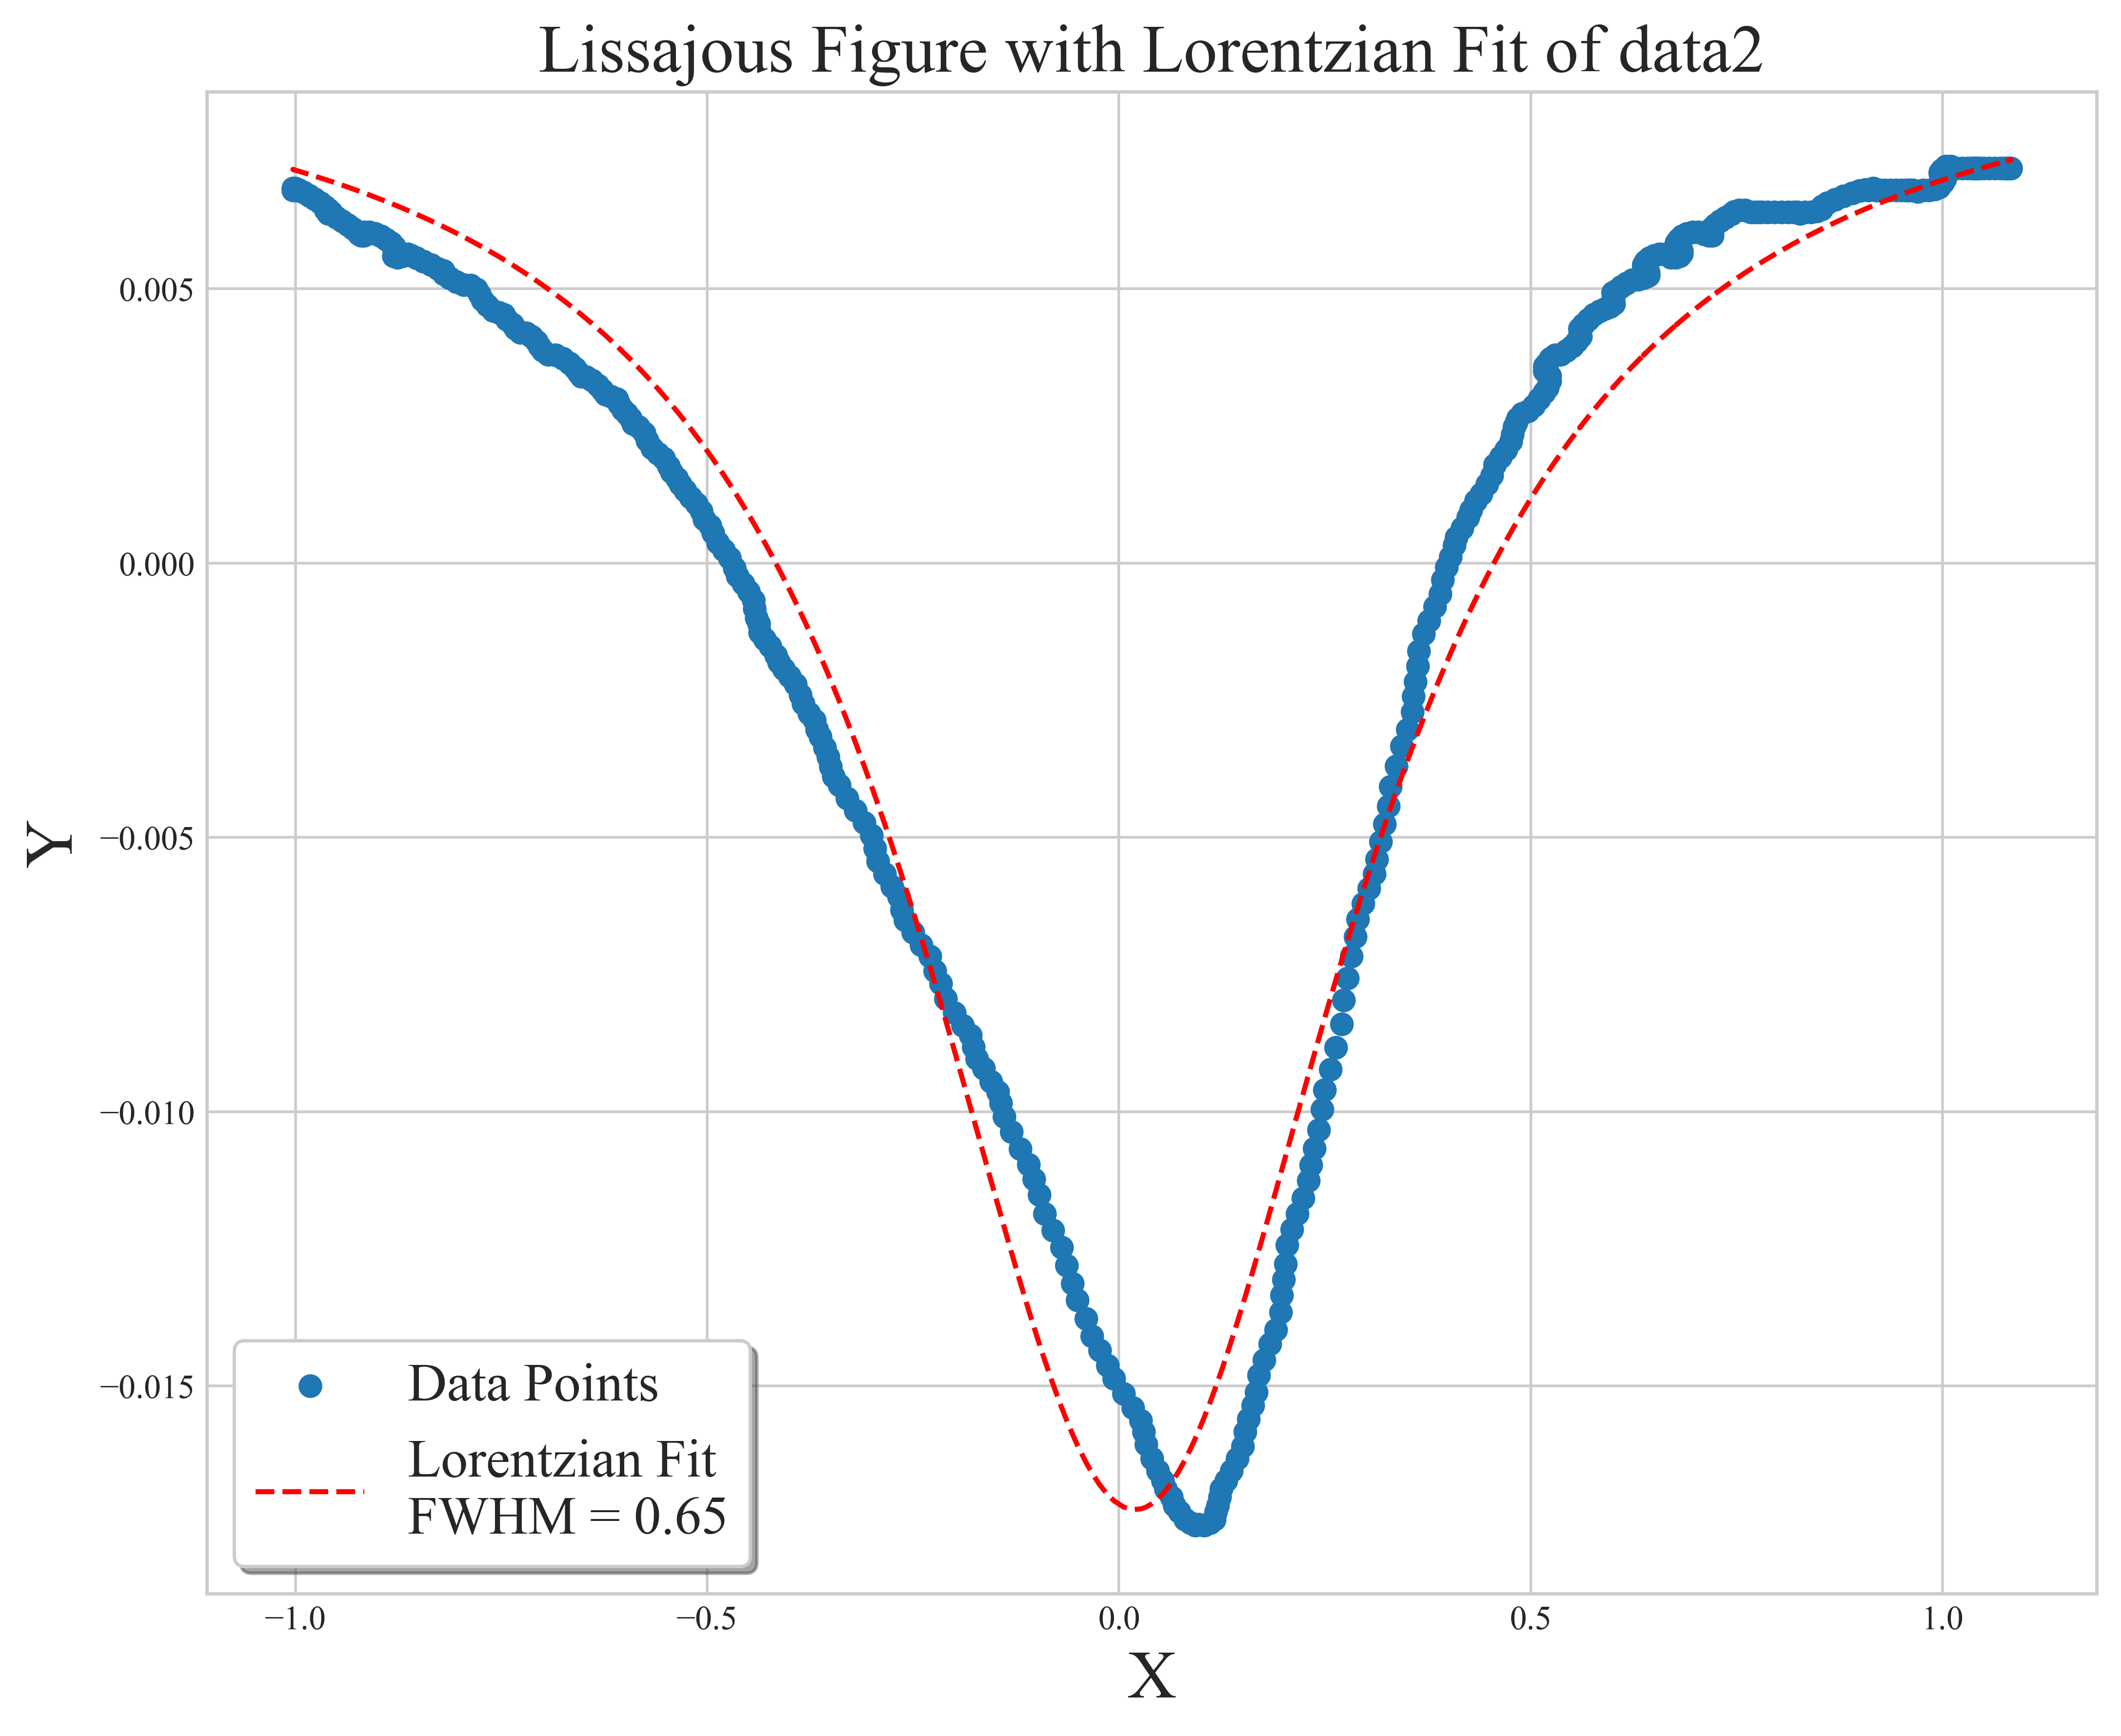
\includegraphics[width=0.7\textwidth]{D4-3-7.png}
			\caption{data2李萨如图拟合}
			\label{fig:D4-3-7}
		\end{figure}
		\begin{figure}[htbp]
			\centering
			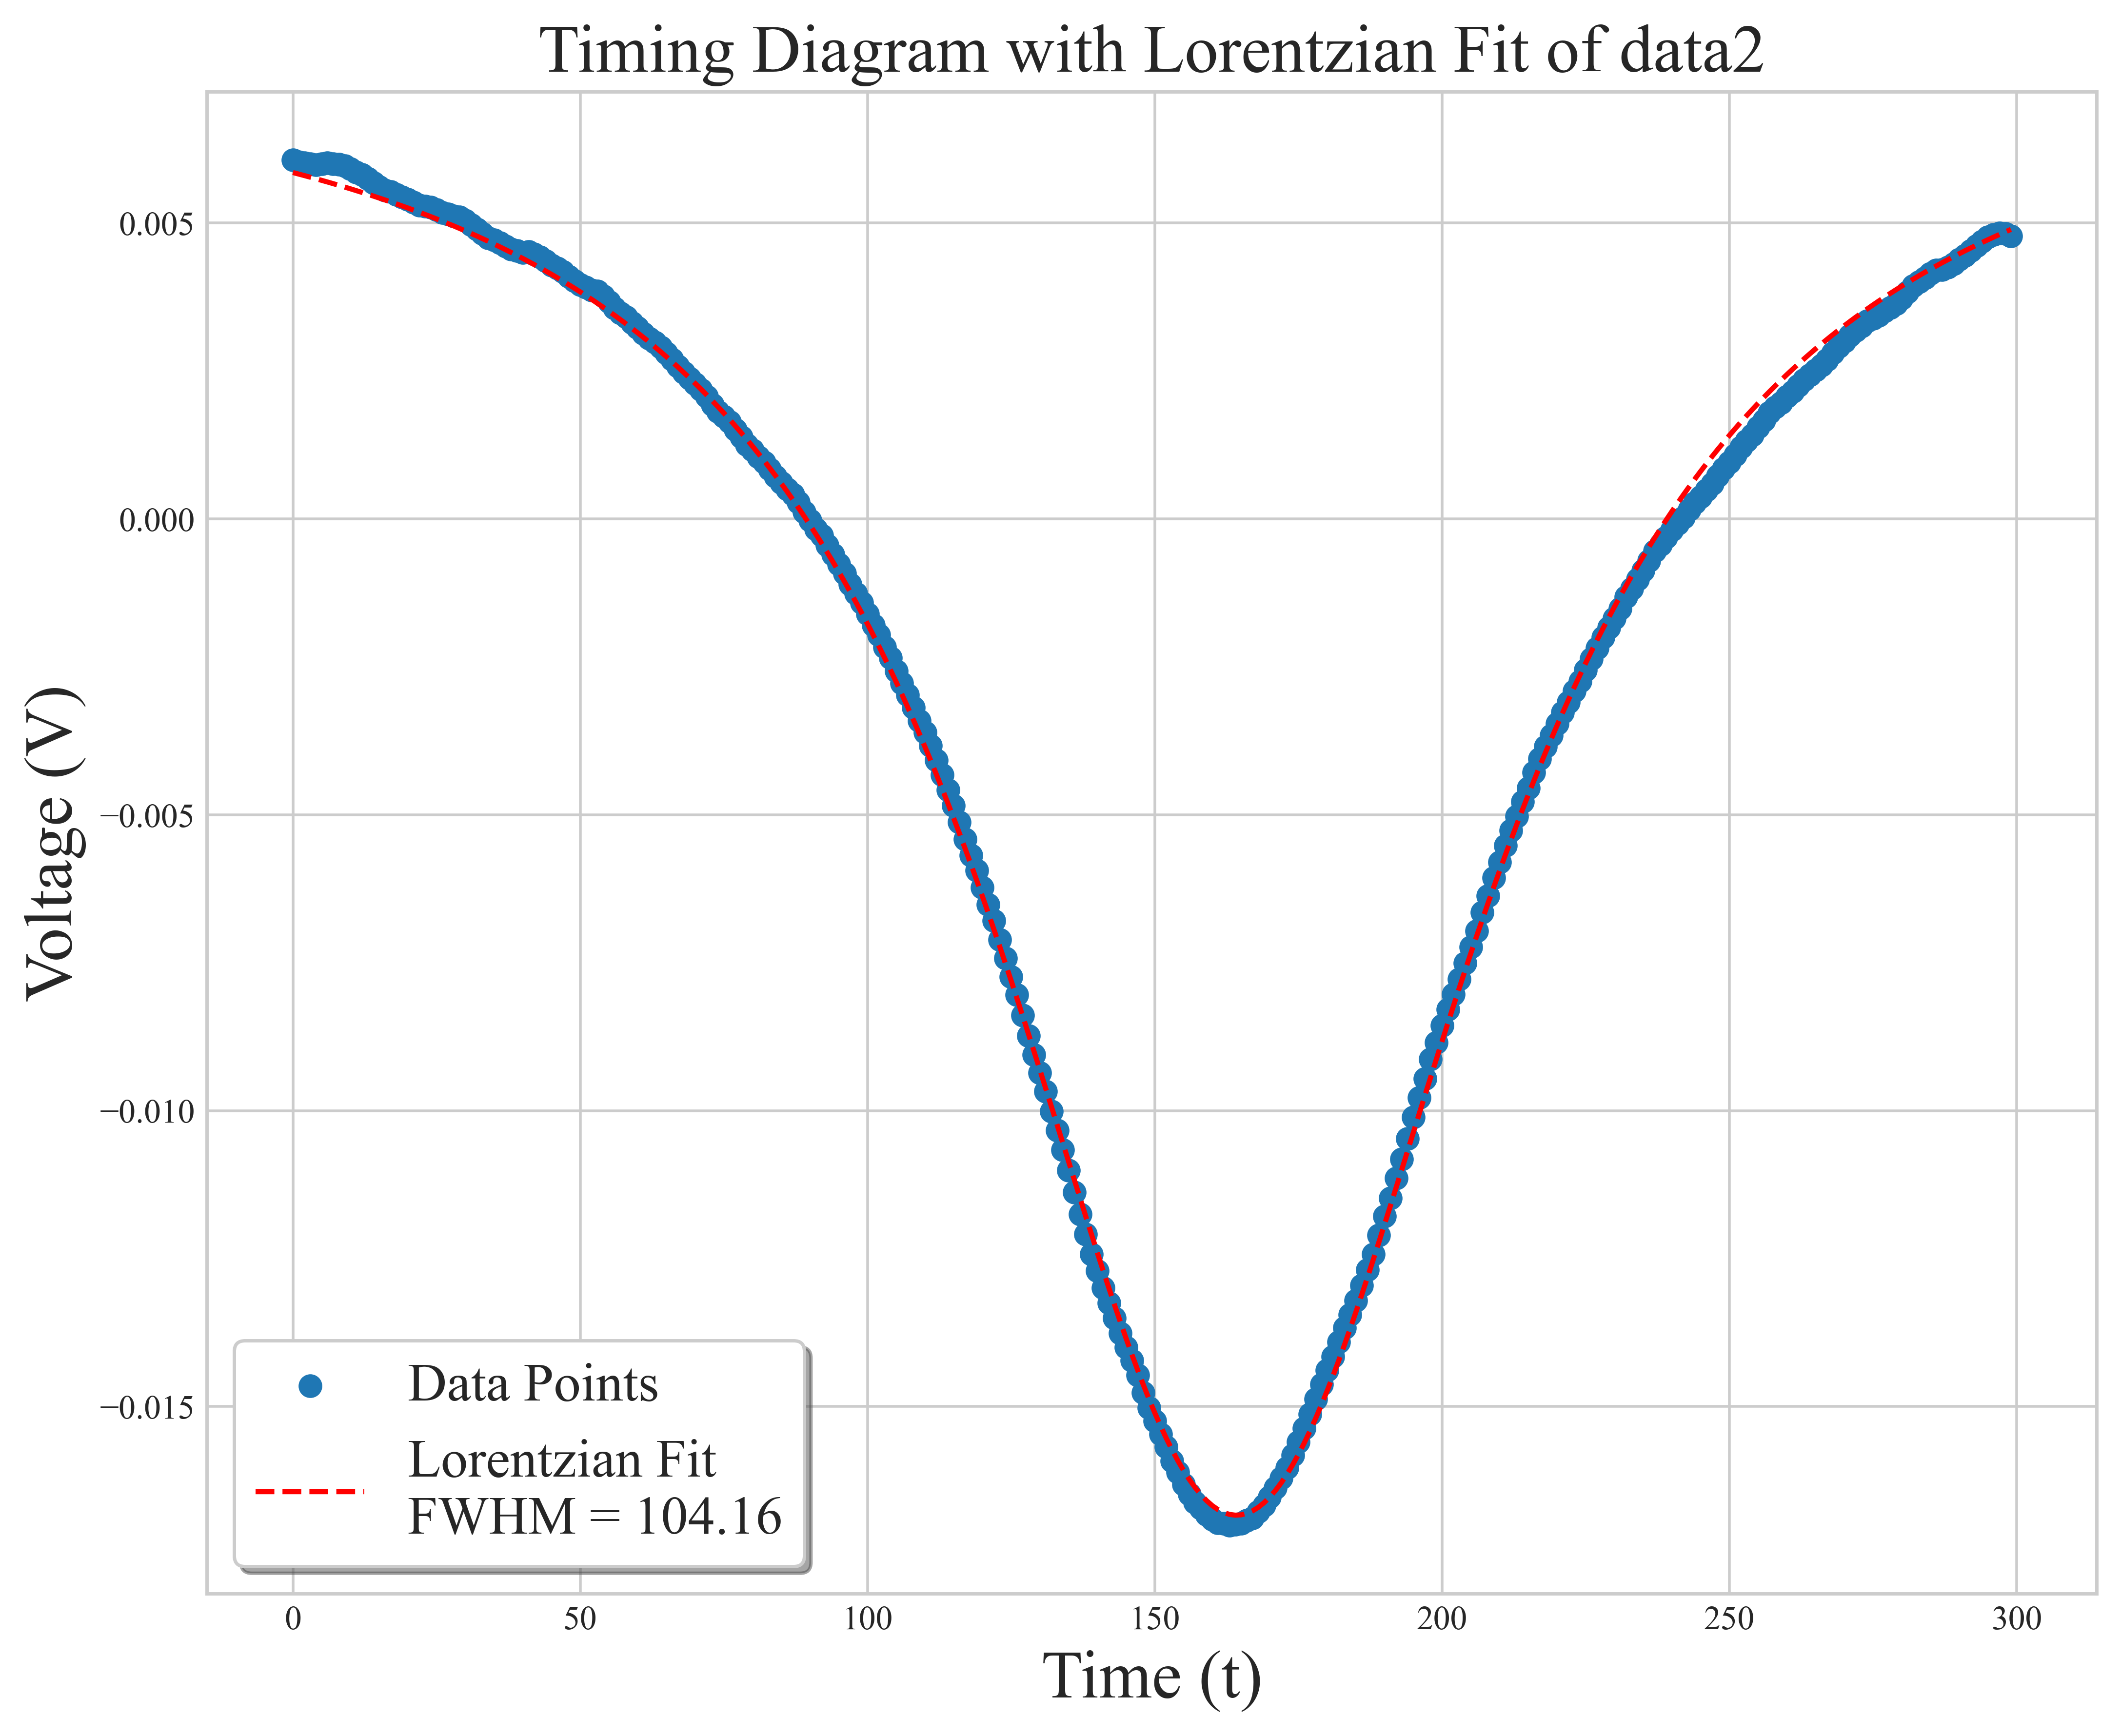
\includegraphics[width=0.7\textwidth]{D4-3-8.png}
			\caption{data2平均时序图拟合}
			\label{fig:D4-3-8}
		\end{figure}

		\begin{enumerate}
			\item data2李萨如图拟合的结果为 FWHM = 0.65,与data1一致,则得到一样的横向弛豫时间$T_2 = 7.2838 \mathrm{ns}$
			\item data2平均时序图拟合的结果为 FWHM = 104.16,得到横向弛豫时间$T_2 = 6.9015 \mathrm{ns}$
		\end{enumerate}









	% \clearpage
	\subsubsection{测量波导波长及微波波长}

		\begin{enumerate}
			\item 由测量到的两个相邻的共振吸收点,可计算得到波导波长为:
				\[
					\lambda_g = 2 (L_2 - L_1) = 46.686 \mathrm{mm}
				\]

			\item 由以下公式可计算得到微波波长,,其中截止波长$\lambda_c = 2a = 45.72 \mathrm{mm}$:
				\begin{align*}
					\lambda_g = \frac{\lambda}{\sqrt{1 - (\lambda / \lambda_c)^2}}	\nonumber	\\
					\Rightarrow	\lambda = 32.6651 \mathrm{mm}	\nonumber	\\
					\Rightarrow f = 9.1778 \mathrm{GHz}	\nonumber
				\end{align*}
		\end{enumerate}

		该测量值明显小于实验中使用的微波频率 9.36GHz。可能是因为在我们改变谐振腔长度时,同时改变了驻波波腹的位置;原本放在驻波波腹位置的样品,在改变谐振腔长度后,偏离了波腹的位置,导致共振吸收信号受到影响(即,示波器显示的共振吸收信号最大的位置,并不对应半波长的整数倍位置)。


	
\clearpage
\subsection{实验后思考题}

% 思考题1
\begin{question}
	观察电子自旋共振需要提供哪些磁场?它们各起什么作用?
\end{question}

	需要提供\textbf{静态磁场}和\textbf{扫场磁场}两种。
	\begin{enumerate}
		\item 在静态磁场的作用下,电子的自旋会发生塞曼能级分裂。其作用是将电子自旋的不同方向对应的能级区分开,使得自旋态能级之间出现差距,从而产生可观察的共振条件。
		\item 扫场磁场用于激发电子的自旋跃迁,当交变磁场频率与自旋态能级分裂的频率相同时,会引发共振吸收。
	\end{enumerate}







	
% 思考题2
\begin{question}
	在电子自旋共振实验中,如何测定共振磁场的大小?测定共振磁场时,应将共振信号调成什么状态?
\end{question}

	\begin{enumerate}
		\item 首先通过高斯计,确定励磁电压与磁感应强度关系曲线。
		\item 随后按照实验二的步骤,调出共振吸收信号。
		\item 再调整励磁电压,使信号均匀出现。由于使用的扫场磁场频率为 50Hz,当两次共振吸收信号间隔为10ms时,一个周期内将出现两次共振吸收,此时静态磁场的大小满足共振吸收条件。
		\item 此时,读出励磁电压大小,并利用实验一得到的励磁电压与磁感应强度关系曲线,即可得到共振磁场大小。
	\end{enumerate}








% 思考题3
\begin{question}
	微波谐振腔的作用是什么?腔长和微波频率的关系是什么?调节短路活塞的作用是什么?实验样品应位于什么位置?为什么?
\end{question}

	\begin{itemize}
		\item \textbf{微波谐振腔}:
			微波谐振腔用于集中微波能量,使得微波在腔内形成驻波,从而在特定位置形成较强的交变磁场,以有效地驱动电子自旋的跃迁,增加信号强度。
		\item \textbf{腔长和微波频率的关系}:
			当谐振腔腔长是半波导波长的整数倍时,谐振腔内可发生谐振:
			\[
				\frac{n}{2} \lambda_g = L \quad n = \pm 1, \pm 2, \cdots
			\]
			而波导波长与入射微波波长存在关系,其中$\lambda_c = 2a$:
			\[
				\lambda_g = 2 (L_2 - L_1) = 46.686 \mathrm{mm}
			\]

		\item \textbf{短路活塞:}
			短路活塞可以在腔体内移动,从而改变腔体的有效长度 。通过调节活塞的位置,可以调节腔体的谐振频率,使其与微波源的频率精确匹配。

		\item 实验样品应放置在腔体内磁场强度最大的位置,通常是驻波波腹的位置。这个位置交变磁场较强,电子受到的驱动也最强,能更有效地引发自旋共振。
	\end{itemize}












\clearpage
\section{D4-1 \quad 电子自旋共振实验 \quad\heiti 实验总结}

	\subsection{实验分工}

		本次实验由\textbf{戴鹏辉}和\textbf{杨舒云}共同完成。
		\begin{enumerate}
			\item 戴鹏辉同学主要完成实验操作、实验报告的撰写。
			\item 杨舒云同学辅助完成实验操作,实验预习报告,实验数据分析。
		\end{enumerate}


	% \subsection{实验心得}
	\subsection{Attachment}
		% The arrangement of the experimental bench desktop is shown in %\cref{}.

		个人签名见 \cref{fig:name1} 、 \cref{fig:name2}.

		\begin{figure}[htbp]
			\centering
			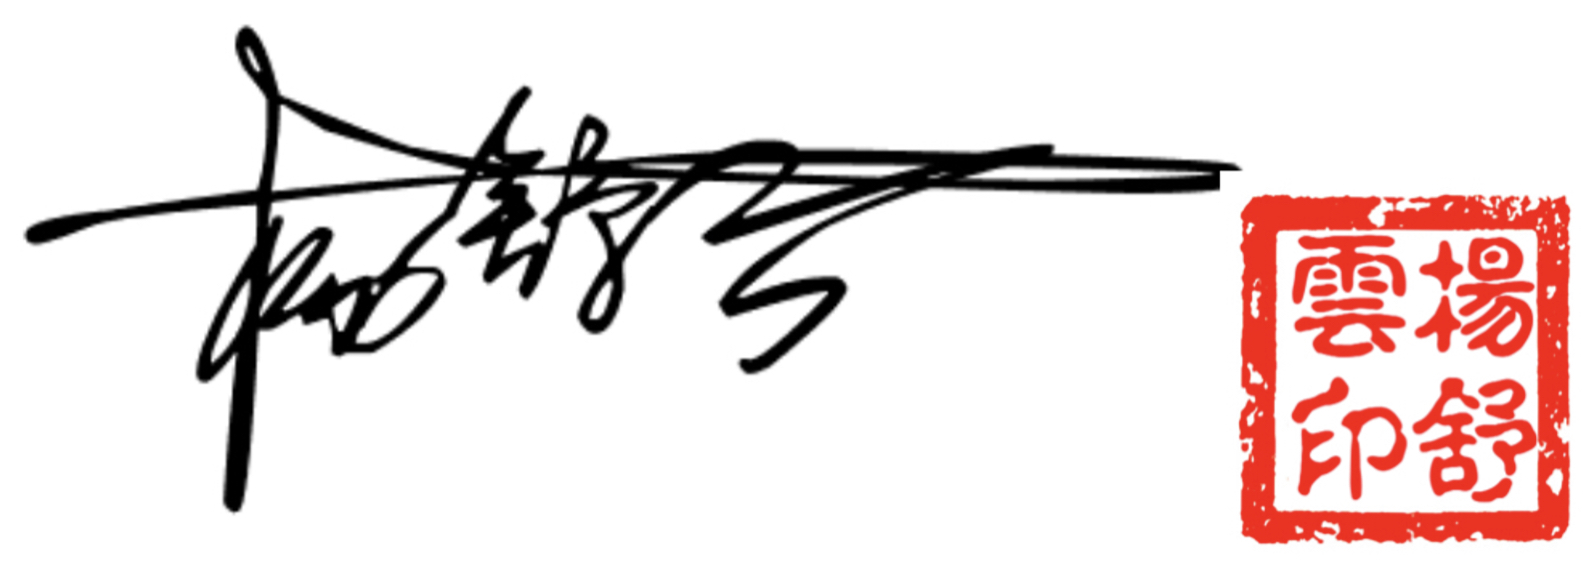
\includegraphics[width=0.5\textwidth]{name.png}
			\caption{signature1}
			\label{fig:name1}
		\end{figure}
		
		\begin{figure}[htbp]
			\centering
			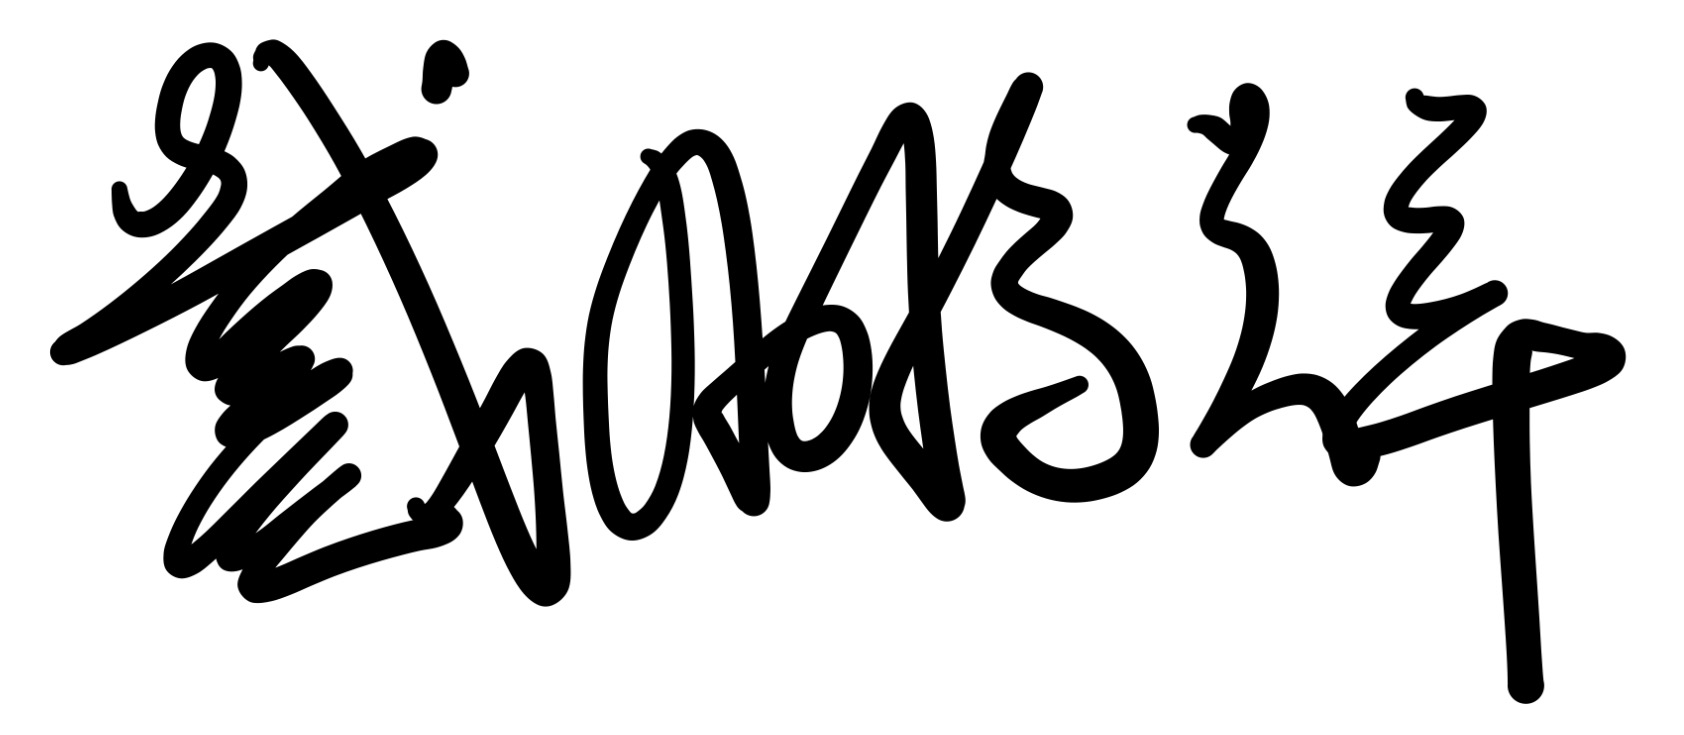
\includegraphics[width=0.35\textwidth]{name-TaLEs.jpg}
			\caption{signature2}
			\label{fig:name2}
		\end{figure}

		% \textbf{All relevant code (Python and LaTex source code) has been uploaded to Github.}

	

	
	


\end{document}
